%% =====================================================================
%% main-llmxive.tex — content-extracted llmXive wrapper
%% =====================================================================
%% Generated by scripts/extract_paper_content.py. The original paper
%% body is preserved; the venue-specific preamble (class, bundled .cls
%% files, custom packages) is DISCARDED and replaced with the llmxive
%% house style + a shim block that no-ops any venue-specific macros the
%% body still references.
%% =====================================================================
\documentclass{llmxive}


%% ── Packages forwarded from original preamble ─────────────────
\usepackage{listings}
\usepackage{amsfonts}
\usepackage{amsmath}
\usepackage{amssymb}
\usepackage{algorithm}
\usepackage{algpseudocode}
\usepackage{enumitem}
\usepackage{siunitx}
\usepackage{url}
\usepackage{xspace}
\usepackage{wrapfig}
\usepackage{placeins}
\usepackage{hyphenat}
\usepackage{parskip}
\usepackage{lipsum}
\usepackage{etoolbox}
\usepackage{ulem}
\usepackage{graphicx}
\usepackage{subcaption}
\usepackage{multirow}
\usepackage[most]{tcolorbox}
\usepackage{natbib}
\usepackage[noabbrev,nameinlink]{cleveref}
\usepackage{pifont}
\usepackage{amsthm}
\usepackage{tabularx}
\usepackage{dsfont}

%% ── Shim layer (venue macros made into no-ops) ────────────────
\makeatletter
\providecommand{\TODO}[1]{}
\providecommand{\abscontent}{}
\providecommand{\absfont}{}
\providecommand{\acknowledgments}{\section*{Acknowledgments}}
\providecommand{\address}[1]{}
\providecommand{\affiliation}[1]{}
\providecommand{\aistatsfinalcopy}{}
\providecommand{\animategraphics}[5][]{\includegraphics[#1]{#3#4}}
\providecommand{\argmax}{\mathop{\mathrm{arg\,max}}}
\providecommand{\argmin}{\mathop{\mathrm{arg\,min}}}
\providecommand{\authornote}[1]{}
\providecommand{\authornotemark}[1][]{}
\providecommand{\authorrunning}[1]{}
\providecommand{\blfootnote}[1]{\footnote{#1}}
\providecommand{\bm}[1]{\boldsymbol{#1}}
\providecommand{\corresponding}{}
\providecommand{\correspondingauthor}[1]{}
\providecommand{\eg}{e.g.,\xspace}
\providecommand{\email}[1]{\href{mailto:#1}{#1}}
\providecommand{\equalcontribution}{}
\providecommand{\etal}{et al.\xspace}
\providecommand{\etc}{etc.\xspace}
\providecommand{\iclrfinalcopy}{}
\providecommand{\icmlfinalcopy}{}
\providecommand{\ie}{i.e.,\xspace}
\providecommand{\iid}{i.i.d.\xspace}
\providecommand{\institute}[1]{}
\providecommand{\keywords}[1]{\par\noindent\textbf{Keywords:} #1}
\providecommand{\neuripsfinalcopy}{}
\providecommand{\orcid}[1]{}
\providecommand{\tablecite}[1]{\cite{#1}}
\providecommand{\theabstract}{}
\providecommand{\titlerunning}[1]{}
\providecommand{\todo}[1]{}
\providecommand{\wrt}{w.r.t.\xspace}
\AtBeginDocument{\renewcommand{\and}{ \textperiodcentered\ }}
\makeatother

%% ── User-defined macros forwarded from original preamble ─────
\makeatletter
\providecommand{\newpara}[1]{\vspace{0.1cm}\noindent\textbf{#1}}
\providecommand{\topfraction}{0.95}
\providecommand{\bottomfraction}{0.95}
\providecommand{\textfraction}{0.03}
\providecommand{\floatpagefraction}{0.85}
\providecommand{\arraystretch}{1.3}
\definecolor{jsonstr}{rgb}{0.5,0.5,0.5}
\definecolor{templatekeyword}{HTML}{E1251B}
\definecolor{templatestring}{HTML}{0B7A75}
\definecolor{templatecomment}{HTML}{6B7280}
\definecolor{templatecodebg}{HTML}{F7F7F8}
\definecolor{jingdongbg}{RGB}{218,41,28}
\definecolor{jingdongred}{RGB}{218,41,28}
\definecolor{jdred}{HTML}{E1251B}
\definecolor{templatefg}{HTML}{1C2B33}
\definecolor{templatebg}{HTML}{F1F4F7}
\definecolor{mygray}{gray}{0.95}
\definecolor{myred}{RGB}{215,48,39}
\definecolor{mygreen}{RGB}{26,152,80}
\definecolor{ForestGreen}{RGB}{34,139,34}
\definecolor{pastelred}{rgb}{1.0, 0.41, 0.38}
\definecolor{redentropy}{HTML}{fff0f0}
\definecolor{best}{HTML}{e8edf2}
\definecolor{secondbest}{HTML}{f3f4f7}
\definecolor{pastelyellow}{RGB}{255,250,205}
\definecolor{LightGray}{HTML}{ebebeb}
\makeatother

%% ── llmXive paper metadata ──────────────────────────────────
\title{JoyAI-VL-Interaction: Real-Time Vision-Language Interaction Intelligence}
\author{Dingyu Yao \and Junhao Zhou \and Chenxu Yang \and Chuanyu Qin \and Haowen Hou \and Zheming Liang \and Congcong Wang \and Yuhang Cao \and Shenglong Ye \and Shuai Xie \and Shuhuan Gu \and Haoyang Huang \and Qingyi Si \and Nan Duan \and Jiaqi Wang}
\paperid{arXiv:2606.14777}
\paperstatus{Preprint}

\begin{document}
\maketitle
\begin{abstract}
Many moments in the real world do not wait for a user to ask. A fire starts on a security monitor, an expression flickers across a video call, or a product a viewer wants flashes by in a livestream. Once missed, the moment is gone, because the physical world does not pause. Yet today’s large models remain mostly turn-based by design: they answer only when addressed, and even video-call apps that appear interactive still operate as question-answer systems, reacting only when polled or prompted. We argue for a different paradigm: a model that is present in the world like a person. It continuously watches what is happening now, decides on its own whether to speak or stay silent, interacts in real time, and delegates to a background model when the problem is hard. This opens a "watch-and-do" mode of human-AI collaboration, expands AI assistance to far more real-life situations, and aligns naturally with the real-time demands of embodied intelligence. To advance interaction models and their adoption across domains, we make two fully open-sourced contributions. First, we release \textbf{JoyAI-VL-Interaction}, an 8B-scale, vision-first VL-interaction model that is proactive by design. The model makes the response decision internally, choosing each second to stay silent, respond, or delegate to a background model, and it excels at vision-triggered responsiveness and time awareness. We pair it with a transferable training recipe, from which capabilities we never trained for emerge, such as guiding a shopper through changing app screens or improvising a lecture from a slide deck. Second, we release a complete, deployable system built around that model. The system streams any ongoing video, from cameras, livestreams, or security feeds, into the model, making it genuinely present in the world. It supports hours of continuous video with sub-second latency. All other components are pluggable, including ASR/TTS modules, memory, visualization UI, and a background brain that can connect to any API, model, or agent.
Across six real-world streaming scenarios, human raters prefer JoyAI-VL-Interaction over the in-app video-call assistants of Doubao and Gemini by a wide margin on both quality and timing, winning 77.6\% against Doubao and 87.9\% against Gemini. To our knowledge, this is the first open, vision-driven interaction model released together with its training recipe, data, and complete deployable system.
With our repository, anyone can deploy an assistant that sees the present, speaks up on its own, and moves fluidly between the physical and digital worlds. 
Our goal is to move VLMs beyond turn-based dialogue toward real streaming interaction, openly and together.
\end{abstract}
\section{Introduction}
\label{sec:introduction}
% todo:我们更擅长什么
% 全双工引用完全：minicpm
% The moments that most need an AI are often the ones no one has time to ask about: a flame on a monitor, an elderly person falling, the very item a shopper wanted gone from the screen in a second. What they share is that the instant worth a word arrives before anyone has thought to ask, and is gone just as quickly. 
The moments that most need AI are often the very moments no one has time to ask for it. 
A toddler wanders toward a hot stove. The decisive play in a match is over before anyone has time to cheer. An aging parent living alone falls in the next room. What these moments share is not merely urgency, but timing: the instant that calls for a word, a cheer, or a steadying hand arrives before anyone thinks to ask, and disappears just as quickly.
Today’s large models are not built for such moments. Most remain fundamentally turn-based: they wait to be addressed, and respond only after they are asked.
% Today's large models are built the wrong way for this. They are almost all turn-based: they wait to be addressed and answer only once asked.
This limitation is structural, not merely a matter of speed. A turn-based model cannot perceive ``now'' by construction: it opens its eyes only at the moment it is prompted. What these situations require instead is a model that continuously sees what is happening in the present and interacts with the world as events unfold.

% Many real situations call for an AI that is present at every moment and responds on its own, with no time for anyone to ask first. A flame leaps up on a monitor, an elderly person falls, or someone walks in where they should not, and an alert must come at once. A scene keeps changing, with slides advancing one by one or a match in play, and the narration has to keep pace. A remote-care feed turns abruptly, or the very item a viewer wanted flashes past in a livestream. What these moments share is simple: the instant worth a word usually arrives before anyone has thought to ask, and it is gone just as quickly. Yet today's large models are almost all turn-based. They wait to be addressed and answer only once asked. What these situations actually need is a model that sees what is happening right now and interacts as it unfolds, but the turn-based paradigm cannot see "now" by construction: it opens its eyes only at the instant it is questioned.

Existing efforts do not truly solve this problem. One line of work is real-time omni models, such as GPT-Realtime-2 \cite{openai2026gptrealtime2} and Qwen3.5-Omni \cite{qwen2026omni}, which are genuinely end-to-end single models (audio and video in; speech out) with low latency and no stitched-together pipeline. 
However, their optimization target remains conversational turn-taking: responding as quickly as possible after the user has spoken. Fundamentally, they are still organized around dialogue. They wait for the user's turn, and are not designed to continuously watch a visual stream and decide on their own when the moment calls for speaking.
Another line of work is consumer video-call products. Doubao's in-app video call \cite{seed2_2026} chases proactivity by firing a background request every few seconds, but its core is still turn-based and its autonomy is locked to the polling cycle: an event is not observed until the next poll, so the system can never react sooner than that interval.
Gemini's in-app video call \cite{gemini31flashlive} goes even less far: it does not perform the background polling that Doubao relies on to monitor for events, and instead remains strictly in a one-question, one-answer interaction pattern.
%and replying only about the frame it sees the instant it is asked. A third line is ...
% We call this gap event latency. 
% Another line is consumer video-call products. Doubao's in-app video call chases proactivity by firing a background request every few seconds, but its core is still turn-based and its autonomy is locked to the polling cycle: an event is not seen until the next poll, so event latency can never fall below that interval. 
% Gemini's in-app video call does not even do this, answering only about the frame it happens to see the instant a question is asked. 
A third line is research on streaming-video understanding \cite{qian2025dispider,qian2025streaming,videollm-online,wang2024mmduet,yan2026proactvl,guan2026videostreamingthinking,awesomevlmstreaming}, which mostly remains at the laboratory stage. It is often evaluated in the manner of offline video understanding \cite{li2025ovobenchfarvideollmsrealworld,lin2024streamingbenchassessinggapmllms}, and it rarely brings together the properties a real-world deployment demands~\cite{yao2026harnessingstreamingvideowild}, namely proactive response\cite{xia2025streamingvideoinstructiontuning,qian2025dispider,yan2026proactvl}, long-horizon memory \cite{yao2025timechatonline,zhang2026hermeskvcachehierarchical,zeng2026streamforest}, and real-time operation \cite{xu2025streamingvlmrealtimeunderstandinginfinite,wang2026acceleratingstreamingvideolarge}. 
It typically advances only one dimension at a time. In short, none of these systems meets the needs of real deployment: each is either turn-driven rather than event-driven, not genuinely present in the live world, or alive only inside a benchmark.

% Existing efforts do not truly solve this. The most capable are the real-time / omni models—GPT-Realtime-2, Qwen3.5-Omni—which are genuinely end-to-end single models (audio, and even video, in; speech out), with low latency and no stitched-together pipeline. But what they optimize is conversational turn-taking—how quickly they answer once you have spoken—and they remain, at heart, organized around dialogue and wait for your turn; they are not designed to watch a visual stream on their own and decide, when no one has asked, whether this is the moment to speak (event latency). A step behind are consumer video-call products: Doubao's in-app video call chases proactivity by firing a background request every few seconds, but its core is still turn-based and its autonomy is locked to the polling cycle—an event is not seen until the next poll, so event latency can never fall below that interval; Gemini's in-app video call does not even do this, answering only about the frame it happens to see the instant a question is asked. A third line, research on streaming-video understanding, mostly remains at the laboratory stage, is often evaluated in the manner of offline video understanding, and does not truly bring together the properties a real-world deployment demands—proactive response, memory, and real-time operation—typically advancing only one of them at a time. In short, none of these meets the needs of real deployment: each is either turn-driven rather than event-driven, not genuinely present, or alive only in a benchmark. 


% \textbf{JoyAI-VL-Interaction} is built for exactly this. We adopt the term interaction model from Thinking Machines Lab (TML) and make its criterion explicit. An interaction model treats whether and when to act as a continuous decision the model makes on its own, judging at each moment whether to respond to the ongoing stream, including speaking when nobody has prompted it. A turn-based model, however low its latency or native its architecture, acts only when a user's turn arrives. The line is not whether turns exist, but whether the model can act unprompted. We and TML in fact reached the same conviction concurrently: for a model to be genuinely present, scalable interactivity must come from the model itself, not be imitated by a harness less capable than the model. Where we differ is that we make vision the first-class driver, and we build the whole thing as an open, deployable system that anyone can adapt.

% \textbf{JoyAI-VL-Interaction} is built for exactly this. We adopt the term interaction model from Thinking Machines Lab (TML) and make its criterion explicit: an interaction model decides on its own, at every moment, whether to act on the ongoing stream, including speaking when nobody has prompted it, whereas a turn-based model acts only when a user's turn arrives, however low its latency or native its architecture. The line is not whether turns exist, but whether the model can act unprompted. We and TML recognized at nearly the same time that interactivity is worth scaling as a capability of its own; where we part is the route to it. TML fuses speech and vision into one large model and shared a research preview; we make vision the first-class driver with speech as pluggable I/O, keep the model compact enough to run on local, low-cost hardware, and open the whole stack so anyone can deploy, reproduce, and build on it.

\textbf{JoyAI-VL-Interaction} is built for exactly this. We adopt the term \textit{interaction model} \cite{thinkingmachines2026interactionmodels} from Thinking Machines Lab (TML) and make its criterion explicit: an interaction model judges for itself, moment to moment, when the time is right to respond to the ongoing stream, the way a person does, choosing when to speak and when to stay silent rather than answering only when addressed. A turn-based model, however low its latency or native its architecture, cannot choose its own moment: it speaks only when a user's turn arrives. The difference is not how fast a model answers, but whether it decides for itself when answering is worth it. We and TML recognized at nearly the same time that interactivity is worth scaling as a capability of its own; where we part is the route to it. TML fuses speech and vision into one large model and shared a research preview; we make vision the first-class driver with speech as pluggable I/O, keep the model compact enough to run on local, low-cost hardware, and open the whole stack so anyone can deploy, reproduce, and build on it.

% \textbf{Contribution 1 — the VL-interaction model.} Our central idea is simple: make \emph{when to act} a learned, per-second decision of the model itself, with staying silent treated as a first-class action alongside speaking and delegating. We turn our base vision-language model, JoyAI-VL-8B (§3.1) into such a vision-first interaction model. Speaking and staying silent are the root of proactivity and time awareness, knowing when a moment is worth a word and when it is not; delegating is how the model reaches for more capability when a problem outgrows real-time inference. We pair every second of the visual stream with the action it calls for, namely time-aligned \cite{thinkingmachines2026interactionmodels}, and the model learns its interactivity from this, as a behavior of its own rather than something bolted on by external turn-detectors or activity heuristics. To keep it affordable over an unbounded stream, we encode the video with AdaCodec, whose cost grows more with how much the scene changes than with frame count (§3.1). We open-source model weight, the full training recipe together with the time-aligned data behind it. Capabilities we never trained for already emerge from it (§5.3), which we read as evidence that the model is acquiring a general watch-and-interact competence rather than scripted tricks, and that time-aligned training is far from saturated. 

\textbf{Contribution 1 — the VL-interaction model.} Our central idea is simple: make when to act a learned, per-second decision of the model itself, with staying silent treated as a first-class action alongside speaking and delegating. We build this vision-first interaction model on our base vision-language model, JoyAI-VL 1.0 (\S\ref{sec:arch}). Speaking and staying silent are the root of proactivity and time awareness, knowing when a moment is worth a word and when it is not; delegating is how the model reaches for more capability when a problem outgrows real-time inference. We pair every second of the visual stream with the action it calls for, yielding time-aligned data, which we construct at scale (\S\ref{sec:data}); from this the model learns its interactivity, as a behavior of its own rather than something bolted on by external turn-detectors or activity heuristics. To keep it affordable over an unbounded stream, we encode the video with AdaCodec\cite{hou2026adacodecpredictivevisualcode}, which spends far fewer tokens on each predictable frame so the budget grows far more slowly over a long stream (\S\ref{sec:arch}). We open-source the model weights, the training recipe, and the data behind it.
% Capabilities we never trained for already emerge, which we read as evidence that the model is acquiring a general watch-and-interact competence rather than scripted tricks, and that this kind of training is far from saturated.

% \textbf{Contribution 1 — the VL-interaction model.} Our central idea is simple: make \emph{when to act} a learned, per-second decision of the model itself, with staying silent treated as a first-class action alongside speaking and delegating. 
% Starting from a language-model base, we train a vision-first VL-interaction model of about 8B parameters and align the visual stream with it at one-second granularity.
% Starting from our base vision-language model, JoyAI-VL-8B (§3.1), we turn it into a vision-first interaction model, trained to act on the visual stream at one-second granularity. 
% At every second the model emits one of three actions on its own: speak, stay silent, or delegate to a background model. Speaking and staying silent are the root of proactivity and time awareness, knowing when a moment is worth a word and, equally, when it is not; delegating is how the model reaches for more capability when a problem exceeds the budget of real-time inference. Crucially, this decision is learned and lives inside the model, not assembled from external turn-detectors or activity heuristics. To keep it affordable over an unbounded stream, we encode the video with AdaCodec, whose cost grows with how much the scene changes rather than with frame count (§3.1). We open-source the full training recipe together with the time-aligned data behind it; because the recipe turns on a single per-second action format rather than any one domain, extending it to a new vertical needs only more streams labeled in the same form. Capabilities we never trained for already emerge from it (§5.3), which we read as evidence that the model is acquiring a general watch-and-interact competence rather than scripted tricks, and that time-aligned training is far from saturated. 

% Contribution 1 — the VL-interaction model. Starting from a language-model base, we train a vision-first VL-interaction model of about 8B parameters and align the visual stream with the model at one-second granularity. At every second the model emits one of three actions on its own: speak, stay silent, or delegate to a background model. Speaking and staying silent are the root of proactivity and time awareness, knowing when a moment is worth a word and, equally, when it is not. Delegating is how the model reaches for more capability when a problem exceeds the budget of real-time inference. This decision is learned in training and lives inside the model; it is not assembled from external turn-detectors or activity heuristics. To keep the model present over an unbounded stream at a budget that vLLM can actually serve, we tokenize the video with AdaCodec, a predictive visual code that spends full vision tokens only where the scene changes and about 16 tokens on each predictable frame in between. We also provide a reproducible training-and-data recipe that transfers to one's own vertical domains. Tellingly, during training we saw abilities with real deployment value emerge that our data never contained, among them guiding a shopper through changing app screens and improvising a lecture from a slide deck. We read this as evidence both that the model is acquiring a general "watch-and-interact" competence rather than scripted tricks, and that our time-aligned training is far from saturated, with substantial headroom as the data scales.



% \textbf{Contribution 2 — the VL-interaction system.} We open-source a complete, deployable system with the interaction model at its center: it is the only component that decides when to speak and when to delegate, while everything else is pluggable and swappable for whatever a deployment needs (your own ASR/TTS, and any API, model, or agent as the background). The system runs two concurrent loops, a real-time loop with the user and an asynchronous loop with the background, joined by the model's ``delegate'' action, and it sustains presence over hours of continuous video on standard serving infrastructure. Because the model is a compact 8B that runs on local, low-cost hardware, the whole stack, the model, the recipe, and the system, can be deployed, fine-tuned, and rebuilt by anyone, not only on large infrastructure.
% In a head-to-head human evaluation across eight everyday scenarios, JoyAI-VL-Interaction is preferred over both Doubao's and Gemini's in-app video-call assistants by a wide margin (§5). 

% \textbf{Contribution 2 — the VL-interaction system.} We open-source a complete system that works out of the box: anyone can feed it a webcam or a livestream, and the interaction model immediately sees what is happening and interacts with the user in real time, genuinely present in the scene. 
% Around the model, the system provides everything a deployment needs, ASR and TTS, a visualization UI, long-horizon memory, and a background bridge, all served on standard vLLM to meet the real-time budget; among them, the interaction model alone decides whether and when to interact, while the rest only transduce and orchestrate around it. 
% Each ships with an open-source default and can be swapped for whatever a deployment needs. Underneath, the model runs two loops at once, joined by its own ``delegate'' action. The first is a real-time loop with the user, in which the model stays present moment to moment, deciding each second whether to speak or stay silent. The second is an asynchronous loop with a background brain: when a problem outgrows real-time inference, the model delegates it there and, crucially, does not go quiet, continuing to watch the scene and talk with the user while the background works, then folding the result back in when it returns. Learning to run both at once, without ever pausing the world it is watching, is what keeps the model present even while a hard task is still pending. In a head-to-head human evaluation across eight everyday scenarios, JoyAI-VL-Interaction is preferred over both Doubao's and Gemini's in-app video-call assistants by a wide margin on quality and timing (§5).

% \textbf{Contribution 2 — the VL-interaction system.} We open-source a complete system that works out of the box: anyone can feed it a webcam or a livestream, and the interaction model immediately sees what is happening and interacts with the user in real time, genuinely present in the scene. Around the model, the system provides everything a deployment needs, ASR and TTS, a visualization UI, long-horizon memory, and a background bridge, all served on standard vLLM to stay real-time over hours of continuous video; among them, the interaction model alone decides whether and when to interact, while the rest only transduce and orchestrate around it. Every component ships with an open-source default and is pluggable, swappable for whatever a deployment needs. The system runs two concurrent loops, joined by the model's ``delegate'' action: a real-time loop with the user, and an asynchronous loop in which the model offloads a hard problem to a background brain while staying present with the user, folding the result back in when it returns. In a head-to-head human evaluation across eight everyday scenarios, JoyAI-VL-Interaction is preferred over both Doubao's and Gemini's in-app video-call assistants by a wide margin on quality and timing (§5).

\begin{figure}[htbp]
    \centering
    
\includegraphics[width=1\textwidth]{pic/overview.pdf}
    \caption{\textbf{JoyAI-VL-Interaction} processes a continuous video stream in real time, deciding at each step whether to respond, stay silent, or delegate complex tasks to a background model for asynchronous handling.}
    \label{fig:overview}
    \vspace{25pt}
\end{figure}

\textbf{Contribution 2 — the VL-interaction system.} We open-source a complete system that works out of the box: anyone can feed it a webcam or a livestream, and the interaction model immediately sees what is happening and interacts with the user in real time, genuinely present in the scene. Around the model, the system provides everything a deployment needs: ASR and TTS, a visualization UI, long-horizon memory, and a background bridge to any API, model, or agent the user brings, all served on standard vLLM to stay real-time over hours of continuous video. Among these, the interaction model alone decides whether and when to interact; the rest only transduce and orchestrate around it. Each ships with an open-source default, and the system provides the hooks to replace it, so a deployment can drop in its own ASR/TTS API or custom modules without rebuilding the stack. The system runs two concurrent loops, joined by the model's ``delegate'' action: a real-time loop with the user, and an asynchronous loop in which the model offloads a hard problem to a background brain while staying present with the user, folding the result back in when it returns. In a head-to-head human evaluation across six everyday scenarios, JoyAI-VL-Interaction is preferred over both Doubao's and Gemini's in-app video-call assistants by a wide margin on quality and timing, winning 77.6\% of comparisons against Doubao and 87.9\% against Gemini. Its strongest margins fall on the most time-critical settings: it wins every comparison in monitoring and alerting against both systems and never loses one in real-time translation or counting, exactly the event-driven, act-at-the-right-moment tasks that turn-based products structurally miss (\S\ref{sec:experiments}).

% \textbf{Contribution 2 — the VL-interaction system.} We open-source a complete, deployable system with the interaction model at its center: it is the only component that decides when to speak and when to delegate, while everything else is pluggable and swappable for whatever a deployment needs (your own ASR/TTS, and any API, model, or agent as the background). The system runs two concurrent loops, a real-time loop with the user and an asynchronous loop with the background, joined by the model's ``delegate'' action, and it sustains presence over hours of continuous video on standard serving infrastructure. Anyone can deploy, fine-tune, and rebuild the whole stack, model, recipe, and system alike, on local, low-cost hardware rather than only on large infrastructure. In a head-to-head human evaluation across eight everyday scenarios, JoyAI-VL-Interaction is preferred over both Doubao's and Gemini's in-app video-call assistants by a wide margin on quality and timing (§5).

% Contribution 2 — the VL-interaction system. We open-source a complete, deployable system with the interaction model at its center. The model is the only component that decides when to speak and when to delegate; everything else is orchestrated around it and is pluggable, free to be swapped for whatever fits a given deployment (ASR/TTS for your own API, and the background for any API, model, or agent you bring). The system runs two concurrent loops, a real-time loop with the user and an asynchronous loop with the background, joined by the model's learned "delegate" action as their seam, and it sustains second-level presence over hours of continuous video through a vLLM-native serving path. By comparison, TML released a research preview of a model; we go further on the system side. At an 8B scale that runs on local and low-cost hardware rather than only on large infrastructure, we open the model, the recipe, and a complete deployable, composable system together, so that anyone can build and adapt their own real-world assistant on top of it.
% Contribution 2 — the VL-interaction system. We open-source a complete, deployable system built around the interaction model at its center: the model is the only component that decides when to speak and when to delegate, while everything else—ASR, TTS, memory, the background brain, the visualization UI—is orchestrated around it and is pluggable, free to be swapped for whatever fits a given deployment (ASR/TTS for your own API; the background for any API, model, or agent you bring). The system runs two concurrent loops—a real-time loop with the user and an asynchronous loop with the background—joined by the model's learned "delegate" action as their seam, and it sustains second-level presence over hours of continuous video through a vLLM-native serving path. By comparison, TML released a research preview of a model; on the system side we go further—opening the model, the recipe, and a complete deployable, composable, community-buildable system together, so that anyone can build and adapt their own real-world assistant on top of it.



% We believe the value here is more than a better "video assistant." When a model can be present in the real world and decide for itself what to watch and when to speak, human–AI collaboration moves from "submit a request and wait" to "watch-and-do"—and AI can step into far more of everyday life, honoring embodied intelligence's premise that the physical world cannot be paused. The same capability—a model that sees for itself and speaks up when it should—is the substrate for a whole class of long-awaited products: a companion that is truly present, AI glasses that see what you see (translating, captioning, and more), an aide that serves as "eyes" for those who cannot see, and many possibilities we have not yet imagined. We are releasing JoyAI-VL-Interaction—the model, its training recipe, and a complete composable system—fully in the open, precisely so the community can keep building on it and explore these possibilities together: new domains, new ways of interacting, an ever-present and self-directed assistant put to new use. To our knowledge, this is the first vision-driven interaction model released as a deployable system; and our larger hope is to move the whole field from turn-based dialogue toward genuine streaming interaction—and to do it in the open.  

The value here is more than a better ``video assistant.'' When a model can be present and decide for itself what to watch and when to speak, human--AI collaboration shifts from ``submit a request and wait'' to ``watch-and-do,'' and AI can step into far more of everyday life, honoring embodied intelligence's premise that the physical world cannot be paused. The same capability is the substrate for a class of long-awaited products: a companion that is truly present, AI glasses that translate or caption what you see, an aide that serves as eyes for those who cannot, and uses no one has imagined yet. We release  JoyAI-VL-Interaction, the model, its training recipe and data, and the full system in the open, precisely so the community can build and explore all of this, and more, together. Our larger hope is to move the field from turn-based dialogue toward genuine streaming interaction, in the open.

% We believe the value here is more than a better "video assistant." When a model can be present in the real world and decide for itself what to watch and when to speak, human–AI collaboration moves from "submit a request and wait" to "watch-and-do," and AI can step into far more of everyday life, honoring embodied intelligence's premise that the physical world cannot be paused. The same capability, a model that sees for itself and speaks up when it should, is the substrate for a whole class of long-awaited products: a companion that is truly present, AI glasses that see what you see and translate or caption it, an aide that serves as "eyes" for those who cannot see, and many possibilities we have not yet imagined. We are releasing JoyAI-VL-Interaction, the model, its training recipe, and a complete composable system, fully in the open, precisely so the community can keep building on it: new domains, new ways of interacting, an ever-present and self-directed assistant put to new use. Our larger hope is to move the whole field from turn-based dialogue toward genuine streaming interaction, in the open. 
% 更多产品可落地的场景，比如，AI眼镜，情侣陪伴
% 机器甚至能感觉被冷落，时间感知
\section{Related Work}

\subsection{Turn-based Models and Products}
\label{sec:product}
Almost all of today's models are \textit{turn-based}: they act only when a user takes a turn, answering once addressed and otherwise idle. This is a structural property, not a matter of speed. A turn-based system has no mechanism for reacting to an event in the world that arrives with no accompanying user utterance, however quickly it can reply once spoken to. Two families of recent systems push hard on responsiveness while keeping this turn-based core.

\paragraph{\textbf{Realtime and omni models.}} OpenAI's GPT-Realtime-2 reasons inside a single speech-to-speech loop \cite{openai2026gptrealtime2}, and Alibaba's Qwen3.5-Omni \cite{qwen2026omni} is a natively pretrained omni-modal model (text, audio, image, video) with real-time streaming and built-in turn-taking and interruption handling, the latter openly released. These remove the latency of cascaded stacks, but what they optimize is \textit{conversational turn-taking}: how quickly and naturally they answer once the user has spoken. Their interaction is organized around dialogue and waits for the user's turn; they are not built to watch a visual stream and decide, unprompted, that this is the moment to speak. Being open, real-time, and multimodal (as Qwen3.5-Omni already is) is therefore necessary but not sufficient for the setting we target.

\paragraph{\textbf{Consumer video-call products.}} In-app ``video call'' features are the most familiar real-time multimodal assistants and our most recognizable baseline, yet their cores remain turn-based. Doubao's runs on ByteDance's Volcano Engine conversational-AI stack, a configurable ASR/VLM/TTS pipeline with stop/turn detection, and its documentation makes the mechanism plain: while no one is speaking, the server only caches incoming video frames and does not send them to the model, so the application must periodically fire an \texttt{ExternalTextToLLM} trigger to obtain any analysis \cite{volcengine2026videounderstanding}; this characterization is based on the publicly available version of the stack, which may differ from the deployed product. ``Monitoring'' is thus an external clock bolted onto a turn-based model: reaction to an on-screen event waits for the next trigger and can never beat the polling interval. Gemini's video call goes less far still; in our use it answers only about the frame visible the instant a question is asked. In neither case does the decision of when to respond live in the model.

% \subsection{Turn-based Models and Products}
% Almost all of today's models are \textit{turn-based}: they act only when a user takes a turn---answering once addressed and otherwise idle. This is a structural property, not a matter of speed; a turn-based system has no mechanism for reacting to an event in the world that arrives with no accompanying user utterance, however quickly it can reply once spoken to. Two families of recent systems push hard on responsiveness while keeping this turn-based core.

% \paragraph{\textbf{ realtime and omni models.}} OpenAI's GPT-Realtime-2 reasons inside a single speech-to-speech loop \cite{openai2026gptrealtime2} , and Alibaba's Qwen3.5-Omni \cite{qwen2026omni} is a natively pretrained omni-modal model (text, audio, image, video) with real-time streaming and built-in turn-taking and interruption handling, the latter openly released. These remove the latency of cascaded stacks, but what they optimize is \textit{conversational turn-taking}---how quickly and naturally they answer once the user has spoken. Their interaction is organized around dialogue and waits for the user's turn; they are not built to watch a visual stream and decide, unprompted, that this is the moment to speak. Being open, real-time, and multimodal---as Qwen3.5-Omni already is---is therefore necessary but not sufficient for the setting we target.

% \paragraph{\textbf{Consumer video-call products.}} In-app ``video call'' features are the most familiar real-time multimodal assistants and our most recognizable baseline, yet their cores remain turn-based. Doubao's runs on ByteDance's Volcano Engine conversational-AI stack---a configurable ASR/LLM/TTS pipeline with stop/turn detection---and its documentation makes the mechanism plain: while no one is speaking, the server only caches incoming video frames and does not send them to the model, so the application must periodically fire an \texttt{ExternalTextToLLM} trigger to obtain any analysis \cite{volcengine2026videounderstanding}. ``Monitoring'' is thus an external clock bolted onto a turn-based model: reaction to an on-screen event waits for the next trigger and can never beat the polling interval. Gemini's video call goes less far still---in our use it answers only about the frame visible the instant a question is asked. In neither case does the decision of when to response live in the model.

% \subsection{Interaction Models}
% A distinct, newer line breaks with the turn-based assumption by moving interactivity \textit{into the model}.

% \paragraph{TML interaction models.} Thinking Machines Lab recently named this an \textit{interaction model} and argued---as we independently and concurrently concluded---that scalable interactivity should come from the model itself rather than an external harness of turn detectors and activity heuristics. Their model handles audio, video, and text in real time and can speak unprompted, acting on the ongoing stream rather than waiting for a user's turn; it was released as a research preview \cite{thinkingmachines2026interactionmodels}. That two groups arrived at this conviction at nearly the same moment we read as a sign that the move from turn-based to interactive models is a direction whose time has come. 

% \paragraph{\textbf{TML interaction models.}} Thinking Machines Lab recently named this an \textit{interaction model} and argued---as we independently and concurrently concluded---that scalable interactivity should come from the model itself rather than an external harness of turn detectors and activity heuristics. Their model handles audio, video, and text in real time and can speak unprompted, acting on the ongoing stream rather than waiting for a user's turn, and---as in our system---it is paired with an asynchronous background model for slower, harder reasoning, the two sharing context; it was released as a research preview \cite{thinkingmachines2026interactionmodels}. That two groups arrived at this approach at nearly the same moment we read as a sign that the move from turn-based to interactive models is a direction whose time has come. Within this shared interaction--background design, our aesthetic differs in two deliberate ways. On modality, rather than fusing audio and vision into the model alike, we keep speech (ASR/TTS) a pluggable module and make vision the model's intrinsic, primary modality for proactive interaction---fitting a watch-and-react setting in which voice is interchangeable I/O. On scale, TML-Interaction-Small is a 276B-parameter mixture-of-experts model (12B active) that its authors describe as the smallest they can serve at the required latency, whereas we deliberately choose a compact $\sim$8B model---balancing interaction-grade responsiveness, local and low-cost deployability, and capability---so that it can be run, fine-tuned, and reproduced widely rather than only on large infrastructure.

% \paragraph{\textbf{Full-duplex speech.}} For speech, Kyutai's Moshi \cite{kyutai2024moshi} is the prominent open instance: a real-time, full-duplex speech--text model in which both sides can speak and listen at once rather than strictly alternating, and the closest open precedent for putting interaction in the model. Its modality and scope---spoken conversation---set it apart from the visual, event-driven setting we address.

% \subsection{Streaming Video Understanding}
% A research line lets models process video as it arrives rather than after the fact, spanning streaming video LLMs, proactive or anticipatory response, and long-horizon video memory [cite, cite, cite]. It is closest to our model contribution, but three gaps separate it from a deployable interaction model. It typically advances one property at a time---responsiveness, \textit{or} proactivity, \textit{or} memory---rather than the three together. It is usually measured on offline benchmarks, at times even in the manner of offline video understanding, which never tests reaction to live events under real-time constraints. And it stops at the model, without the surrounding system---serving, memory, transduction, delegation---that hours of sustained real-time presence demand.

% \subsection{Our Position.} Read along two axes---\textit{how} a model interacts and \textit{what} is released---JoyAI-VL-Interaction occupies a cell no prior work does. Against turn-based systems, native or product, the decision of when to act lives inside our model and is taken every second, event-driven, so reaction is bounded by inference rather than by a user's turn or a trigger clock. Against TML's interaction model, we make \textbf{vision} the first-class driver---the watch-and-react setting rather than audio--video conversation---and we open-source not a research preview but the model, its training recipe, and a complete, composable, deployable system. Against Moshi, we are vision-driven rather than speech-centric, reacting to events that carry no conversational turn at all. And against streaming-video research, we bring responsiveness, proactivity, and memory together in one model and run it inside a system built for sustained presence. To our knowledge, JoyAI-VL-Interaction is the first open, vision-driven interaction model released together with a complete deployable system---the point where all of these properties meet, rather than any one alone.

\subsection{Interaction Models}
A distinct, newer line breaks with the turn-based assumption by moving interactivity into the model.
\paragraph{\textbf{TML interaction models.}} Thinking Machines Lab recently named this an \textit{interaction model} and argued, as we independently and concurrently concluded, that scalable interactivity should come from the model itself rather than an external harness of turn detectors and activity heuristics. Their model handles audio, video, and text in real time and can speak unprompted, acting on the ongoing stream rather than waiting for a user's turn, and, as in our system, it is paired with an asynchronous background model for slower, harder reasoning, the two sharing context; it was released as a research preview \cite{thinkingmachines2026interactionmodels}. That two groups arrived at this approach at nearly the same moment we read as a sign that the move from turn-based to interactive models is a direction whose time has come. Within this shared interaction--background design, our aesthetic differs in two deliberate ways. On modality, rather than fusing audio and vision into the model alike, we keep speech (ASR/TTS) a pluggable module and make vision the model's intrinsic, primary modality for proactive interaction, fitting a watch-and-interact setting in which voice is interchangeable I/O. On scale, TML-Interaction-Small is a 276B-parameter mixture-of-experts model (12B active) that its authors describe as the smallest they can serve at the required latency, whereas we deliberately choose a compact $\sim$8B model (balancing interaction-grade responsiveness, local and low-cost deployability, and capability) so that it can be run, fine-tuned, and reproduced widely rather than only on large infrastructure.
\paragraph{\textbf{Full-duplex speech.}} For speech, Kyutai's MoshiRAG \cite{chien2026moshiragasynchronousknowledgeretrieval} is the prominent open instance: a real-time, full-duplex speech--text model in which both sides can speak and listen at once rather than strictly alternating, and the closest open precedent for putting interaction in the model. Its modality and scope (spoken conversation) set it apart from the visual, event-driven setting we address.


\subsection{Streaming Video Understanding}
A research line lets models process video as it arrives rather than after the fact, spanning streaming video LLMs, proactive response \cite{xia2025streamingvideoinstructiontuning,qian2025dispider,yan2026proactvl}, real-time inference \cite{xu2025streamingvlmrealtimeunderstandinginfinite,wang2026acceleratingstreamingvideolarge}, and long-horizon video memory \cite{yao2025timechatonline,zhang2026hermeskvcachehierarchical,zeng2026streamforest}. It is closest to our model contribution, but three gaps separate it from a deployable interaction model. It typically advances one property at a time (responsiveness, \textit{or} proactivity, \textit{or} memory) rather than the three together. It is usually measured on offline benchmarks, at times even in the manner of offline video understanding, which never tests reaction to live events under real-time constraints. And it stops at the model, without the surrounding system (serving, memory, transduction, delegation) that hours of sustained real-time presence demand. 
% 丁钰师妹辛苦了！

\subsection{Our Position.} Read along two axes, \textit{how} a model interacts and \textit{what} is released, JoyAI-VL-Interaction occupies a cell no prior work does. Against turn-based systems, native or product, the decision of when to act lives inside our model and is taken every second, event-driven, so reaction is bounded by inference rather than by a user's turn or a trigger clock. Against TML's interaction model, we make vision the first-class driver, the watch-and-interact setting rather than audio--video conversation, and we open-source not a research preview but the model, its training recipe, and a complete, composable, deployable system. Against MoshiRAG, we are vision-driven rather than speech-centric, reacting to events that carry no conversational turn at all. And against streaming-video research, we bring responsiveness, proactivity, and memory together in one model and run it inside a system built for sustained presence. To our knowledge, JoyAI-VL-Interaction is the first open, vision-driven interaction model released together with a complete deployable system: the point where all of these properties meet, rather than any one alone.



\section{JoyAI-VL-Interaction Model} \label{sec:model}


Figure~\ref{fig:overview} summarizes the model. JoyAI-VL-Interaction watches a streaming visual input and, at every second, takes one of three actions: speak to the user, stay silent and keep watching, or delegate a slower, harder task to an asynchronous background model whose result is folded back into the stream when ready. The first two actions form a real-time loop with the user; the third, an asynchronous loop with the background.



\begin{figure}[t]
\vspace{-1.3\baselineskip}
\centering
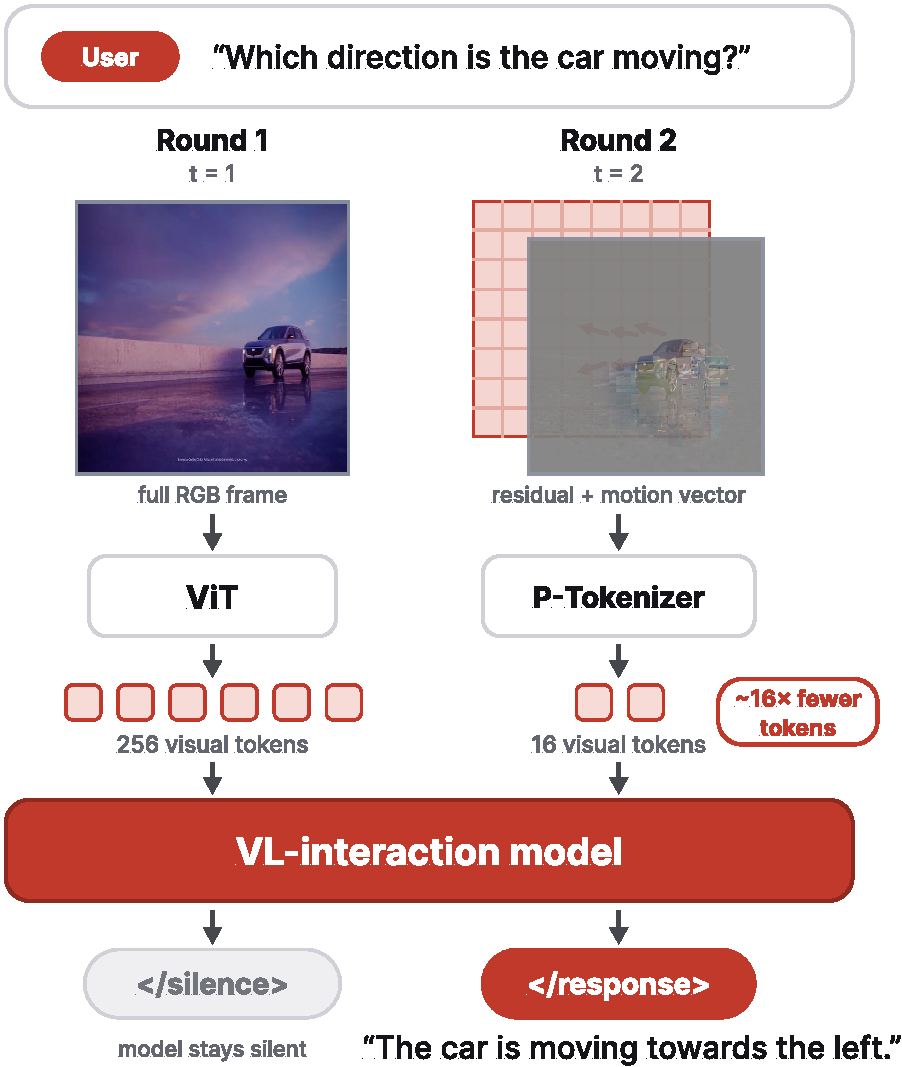
\includegraphics[width=0.44\textwidth]{./pic/adacodec-streaming-dialogue.pdf}
% \caption{\textbf{Model overview and a streaming dialogue.} At each step the model reads the incoming video and decides to stay silent (\texttt{</silence>}) or respond (\texttt{</response>}). Video is encoded with AdaCodec: a reference frame spends full ViT tokens (256), while each predictable frame is coded from motion and residuals into $\approx$16 P-tokens ($\sim$16$\times$ fewer). In the streaming example, the model stays silent on the first frame and answers once the next frame reveals the car's motion.}
\caption{Model overview and video encoding with AdaCodec~\cite{hou2026adacodecpredictivevisualcode}.}
\label{fig:adacodec}
\vspace{-3\baselineskip}

\end{figure}


Two design points frame the rest of this section. First, the model learns a background-agnostic delegation protocol, so the background can be swapped for any external model, agent, or API; we cover the model side here and the system side in \S\ref{sec:system}. Second, the model does not process or generate speech itself: turning voice into text and back is left to pluggable ASR/TTS in the system, keeping the autonomous, vision-driven core decoupled from interchangeable I/O.



% Two design points frame the rest of this section. First, the model learns a background-agnostic delegation protocol, so the background can be swapped for any external model, agent, or API; we cover the model side here and the system side in \S\ref{sec:system}. Second, vision is the model's only in-model modality: it perceives visual input together with text and emits a decision and, when it speaks, a textual response. It does not process or generate speech itself; turning voice into text and back is left to pluggable ASR/TTS in the system, keeping the autonomous, vision-driven core decoupled from interchangeable I/O.

% The section then builds the model from this behavior outward: the architecture and pre-training (\S\ref{sec:arch}), the data that teaches when to speak, stay silent, and delegate (\S\ref{sec:data}), and the training recipe (\S\ref{sec:recipe}), which covers mid-training, the training objective, reinforcement learning, and infrastructure.



The rest of the section builds the model from this behavior outward: the base model and architecture (\S\ref{sec:arch}), the data that teaches when to speak, stay silent, and delegate (\S\ref{sec:data}), and the training recipe (\S\ref{sec:recipe}), which covers continue training, the training objective, reinforcement learning, and infrastructure.




\subsection{JoyAI-VL 1.0 and Architecture}
\label{sec:arch}

% \paragraph{\textbf{Initialization and pre-training.}}
% JoyAI-VL-Interaction is built on a standard vision-language backbone that we then turn into an interaction model. The language model is initialized from Qwen3-8B, the visual encoder is the Qwen3-VL ViT (400M parameters), and the projection layer between them is trained from scratch. On this stack we run two stages, representation alignment (116 million tokens) and vision-language pre-training (400 billion tokens), to obtain our base model, JoyAI-VL-base. At this point the model is a conventional, turn-based VLM. Its per-second interaction behavior, deciding each second whether to speak, stay silent, or delegate, is acquired afterward through the mid-training and post-training of \S\ref{sec:recipe}.


\paragraph{\textbf{JoyAI-VL 1.0.}}
JoyAI-VL-Interaction is built on JoyAI-VL-1.0, %a standard vision-language backbone that we then turn into an interaction model. 
where the language model is initialized from Qwen3-8B \cite{yang2025qwen3technicalreport}, the visual encoder is the Qwen3-VL ViT \cite{bai2025qwen3vltechnicalreport}, and the projection layer between them is trained from scratch. JoyAI-VL 1.0 is obtained through three stages, representation alignment, vision-language pre-training and post-train with On-Policy Distillation \cite{lu2025onpolicydistillation} and RL \cite{liu2026gdpogrouprewarddecouplednormalization,shao2024deepseekmathpushinglimitsmathematical}. At this point the model is a conventional, turn-based VLM. Its per-second interaction behavior, deciding each second whether to speak, stay silent, or delegate, is acquired afterward through the interaction-training recipe in \S\ref{sec:recipe}.



\paragraph{\textbf{Native Streaming Video Codec.}}
We tokenize the video stream with AdaCodec~\cite{hou2026adacodecpredictivevisualcode} (Figure~\ref{fig:adacodec}), a predictive visual code inspired by predictive coding and video codecs: instead of re-encoding every frame, it transmits only what prediction cannot explain. It spends full ViT tokens only on reference frames and encodes the predictable frames in between as compact P-tokens built from motion and residuals, so the model reads an interleaved stream of reference tokens and P-tokens rather than a sequence of full RGB frames. A predictive-cost reset opens a new reference frame whenever prediction becomes costly, placing reference frames exactly where the scene changes enough to need them. This matches our setting directly: a present, always-watching model must consume an unbounded video stream, where a per-frame interface spends full ViT tokens on every frame, so cost and latency grow quickly with the length of the stream. AdaCodec spends only about 16 tokens on each predictable frame and full ViT tokens only at scene changes, so the budget grows far more slowly and its heavy part scales with how much the scene changes rather than with frame count.





\subsection{Data Construction for VL-Interaction }
\label{sec:data}

The applications we build for share a single demand: the assistant must be present and act on its own, at the moment that matters, with no one there to prompt it. A security feed where a flame has just appeared, a livestream where the item a viewer wants is flashing past, AI glasses that should caption or translate what is in front of you the instant it appears, a companion that should speak up only when there is something worth saying. In each case the right moment to act is set by the world, not by the user, and a model that waits to be addressed has already missed it. The data in this section is built to give the model exactly the abilities these settings demand: to watch a visual stream continuously and decide for itself, second by second, whether to speak, stay silent, or hand a hard problem to a heavier background model; to act on what it sees rather than wait to be asked; and to keep track of time, so that it knows not just what is happening but when. Teaching these abilities broadly, rather than for any single use case, is the goal of everything that follows. 

Concretely, at each one-second step the model takes one of three actions over the visual stream seen so far: it can stay silent and keep watching, emitting a \texttt{</silence>} token; speak, emitting a \texttt{</response>} token and a textual reply; or delegate a slower, harder subtask to an asynchronous background model. Delegation follows a fixed, background-agnostic protocol defined over text requests and results, so any external model, agent, or API can serve as the background (\S\ref{sec:system}). We teach these three decisions at one-second granularity, over and over, across as much of real life as we can capture.

\paragraph{\textbf{Capabilities the data covers.}}
To span this range, the data comprises more than 4M time-aligned streaming clips organized into six families. The first five are: (1) proactive alerting and anomaly detection on live feeds; (2) time-aligned question answering in backward, present, and forward timing; (3) counting and perception over time; (4) live commentary and narration; and (5) multi-turn casual chat in a variety of styles, ranging from everyday conversation over egocentric short video, to extended dialogue across long videos, to companionship-style exchanges. The sixth (6) cuts across all of the others: delegation episodes pair the ongoing scene with hard, off-stream subtasks—video-grounded knowledge questions, STEM problems, and video reasoning problems—that the model should route to the background rather than answer inline. A single per-second action format applies across every family, so each scenario jointly teaches the model when to speak, when to stay silent, and, where appropriate, when to delegate.

\paragraph{\textbf{Constructing time-aligned data.}}
Per-second supervision is what makes this behavior learnable, and it is costly to obtain at scale. Every example must be right along two axes: content, what the model says when it speaks, and timing, the exact second at which it should speak, stay silent, or delegate. Silence is a first-class label rather than the absence of one, since most steps in any stream should be silent and the model must learn to wait instead of speaking at every step. To get both axes right at scale, we run a multi-stage pipeline with dedicated verifier agents, and we deliberately favor quality over quantity. Each candidate example is checked at two levels: globally, over all input frames together with the full annotation, and locally, over the frames at the annotated timestamp and the reply tied to them. An example is admitted only if it passes both checks, and is discarded the moment it fails either. Each source is annotated along whichever axis is its bottleneck, and only examples that survive every check enter the corpus, so heterogeneous raw material is funneled into one clean, consistent per-second action format.

We tailor the construction to each family. For offline video-QA, the content of open-source data is already trustworthy, so the work is almost entirely about timing: a larger VLM marks when the evidence relevant to each question appears, and we form three timing types around it. In a backward example the question is asked after the evidence has appeared and the model responds at the moment the question arrives; in a present example the question is asked just as the evidence appears and the model responds at that moment; in a forward example the question is asked before the evidence appears and the model stays silent until the evidence arrives, then responds at that instant. For multi-turn casual chat, the casual nature of the exchange keeps the bar on content low, so we prioritize timing instead. Two VLM agents converse over a continuously playing video, one asking questions grounded in what it currently sees while the other watches the same stream and answers. To place each turn in time, we sample a time point at random and give the annotating model only the three frames around that point, which anchors every response to its timestamp and prevents large timing drift; a verifier agent then screens each exchange for grounding and quality. 

For commentary and narration, the commentator's authentic style is itself the value, so rather than synthesize it we collect open-source commentary and broadcast footage and recover the real spoken content with ASR, which preserves the natural cadence of when a person speaks and pauses and yields realistic silence labels. For counting, we run two passes over a counting-oriented source: the first keeps only videos in which objects reappear, and the second lays down the per-second labels. For perception over time, we insert time-conditioned content into ready-made multi-turn dialogues: for instance, requiring in the question that the answer be withheld for a precise interval before it is given, adding an instruction that increments a running count by one every $n$ seconds, or bounding the time window within which a question and its answer may occur; these rules yield exact, checkable timing without further manual annotation. 

 For alerting and anomaly detection, timing accuracy matters most, since an alert one second late describes a different moment, so we build this data from two sources. From open-source temporal-grounding annotations we convert directly into per-second labels, with a verification pass over the onsets. For web-collected videos, which carry no annotations, the pipeline proposes a candidate trigger window and tightens it through several stages: it filters videos to viable candidates, samples a window, generates and hard-filters a target by type, and applies a window-level verifier; a dense precheck then scans every 1 fps frame from the query time to the candidate trigger and discards the example if the target appeared earlier, so the alarm marks a genuine first onset, after which we localize the trigger to a single frame.

\paragraph{\textbf{Anatomy of a delegation episode.}}
Delegation is the most intricate behavior in the corpus, and the most distinctive: it is where the model learns to recognize the limits of real-time inference and hand off, mid-stream, to a heavier background brain without ever pausing the world it is watching. Each episode is built end to end, pairing a trigger (a subtask the model should not solve inline) with a written request and a returned result, and we synthesize these episodes three ways: (i) inserting ready-made pure-text hard problems such as STEM questions, where it is the difficulty rather than the modality that should send them to the background; (ii) converting open-source offline video-reasoning problems and using a large model to weave them into annotated multi-turn chat, so a genuinely hard visual question can surface naturally in the middle of a conversation; and (iii) synthesizing full episodes with a multi-role agent pipeline, in which a Planner scripts the episode, a Timestamp / Visual Verifier runs multi-level checks, over the whole clip and at the trigger frame, that the trigger and its timing are grounded in what is actually on screen, a Background agent produces the heavy answer, and a Foreground Rewriter turns it into a natural reply.


At the heart of the episode is the two-loop choreography it teaches. The instant the model decides to delegate, it does not go quiet. It first hands the user a brief holding reply (for example, ``let me look into that''), then emits a hidden delegate token and query that the user never sees, dispatching the hard subtask to the background while the visual stream keeps rolling. We then inject a random delay that simulates the background's variable reasoning time, and only after that delay is the result folded back in, at which point the model produces its formal answer in context. The delay is the whole point: by varying it, we force the model to stay present while a delegation is still pending, continuing to watch the scene, field new turns, and hold its silence when nothing is worth saying, rather than freezing until the background returns. This is the exact seam where the real-time loop with the user and the asynchronous loop with the background are stitched together, and the model learns to run both at once. Across all six families, however different their raw material, every construction is reduced to the same per-second labels of silence, response, and delegation and passes through the same multi-level verification, which is what lets such heterogeneous sources train a single, unified interaction policy.

\paragraph{\textbf{A transferable recipe, and signs of emergence.}}
Because the construction is defined by this common per-second format rather than by any one domain, the recipe transfers cleanly to new scenarios: adding a capability is as simple as supplying streams from that domain, annotated in the same per-second form and passed through the same verifiers, with no change to architecture or training objective. And the payoff scales. Even a modest amount of time-aligned data is enough for strong interaction behavior to emerge, a sign that the recipe is highly data-efficient and that time-aligned training is nowhere near saturated, with substantial headroom still ahead as the data grows. Most strikingly, capabilities we never explicitly trained for emerge on their own, including guiding a user through a purchase across changing app screens and improvising a full lecture from a slide deck. We read this as strong evidence that the model is acquiring a general watch-and-interact competence rather than memorizing scenario-specific tricks, and that the same recipe can grow the next generation of always-present assistants, from AI glasses that narrate what you see to companions and accessibility aides that serve as eyes for those who cannot. What we have seen so far is only the beginning. 




% \subsection{VL interaction data}
% \label{sec:data}

% At each one-second step, the model takes one of three actions over the visual stream seen so far: stay silent and keep watching, emitting a \texttt{</silence>} token; speak, emitting a \texttt{</response>} token and a textual reply; or delegate a slower, harder subtask to an asynchronous background model. Delegation follows a fixed, background-agnostic protocol defined over text requests and results, so any external model, agent, or API can serve as the background (\S\ref{sec:system}).

% \paragraph{\textbf{Capabilities the data covers.}}
% % To learn this behavior broadly rather than for a single use case, the data spans a range of streaming scenarios: monitoring and alerting on live feeds; time-aware question answering; counting and perception over time; live narration and guidance, such as event commentary and step-by-step how-to; and multi-turn question answering and temporal reasoning about the ongoing scene. Across all of them the same per-second action format applies, so every scenario also teaches the model when to speak, when to stay silent, and, where appropriate, when to delegate.
% To learn this behavior broadly rather than for a single use case, the data totals more than 2M time-aligned streaming clips, organized into several families: proactive alerting and anomaly detection on live feeds; time-aligned question answering in backward, present, and forward timing; counting and perception over time; live commentary and narration; and multi-turn casual chat in a range of styles, including everyday conversation over egocentric short video, extended dialogue across long videos, companionship-style exchanges. Cutting across all of these, delegation episodes pair the ongoing scene with hard, off-stream subtasks, including video-grounded knowledge questions, STEM problems, and video reasoning problems, that the model should route to the background rather than answer inline. Across all of them the same per-second action format applies, so every scenario also teaches the model when to speak, when to stay silent, and, where appropriate, when to delegate.


% \paragraph{\textbf{Constructing time-aligned data.}}
% Per-second supervision is what makes this behavior learnable, and it is costly to obtain at scale. Every example must be right along two axes: \emph{content}, what the model says when it speaks, and \emph{timing}, the exact second at which it should speak, stay silent, or delegate; silence is a first-class label rather than the absence of one, since most steps in any stream should be silent and the model must learn to wait instead of speaking at every step. 

% Because different sources are reliable on different axes, we tailor each construction to whichever axis is its bottleneck and cast all of them into the same per-second action format. For offline video-QA, the content of open-source data is already trustworthy, so the work is almost entirely about timing: a larger VLM marks when the evidence relevant to each question appears, and we form three timing types around it. In a backward example the question is asked after the evidence has appeared and the model responds at the moment the question arrives; in a present example the question is asked just as the evidence appears and the model responds at that moment; in a forward example the question is asked before the evidence appears and the model stays silent until the evidence arrives, then responds at that instant; every other step is labeled silence, and Figure~\ref{fig:timealign} shows one example of each. For multi-turn casual chat, the content carries a lower correctness bar, so we reverse the order and fix timing first and then fill in content: two VLM agents converse over a continuously playing video, one asking questions grounded in what it currently sees while the other watches the same stream and answers, with verifier agents in the pipeline to screen the result. For commentary and narration, the commentator's authentic style is itself the value, so rather than synthesize it we collect open-source commentary and broadcast footage and recover the real spoken content with ASR, which preserves the natural cadence of when a person speaks and pauses and yields realistic silence labels. For counting and perception over time, we run two passes over a counting-oriented source: the first keeps only videos in which objects reappear (the harder case the model must track across time), and the second lays down the per-second labels. For alerting and anomaly detection, timing accuracy matters most, since an alert one second late describes a different moment, so we convert open-source temporal-grounding annotations into per-second labels and add a model-based verification pass over the converted onsets. For delegation, each episode is built end to end, pairing a trigger the model should not solve inline with a written request and a returned result, and we construct it three ways: (i) inserting ready-made pure-text hard problems such as STEM questions that are independent of the video; (ii) converting open-source offline video-reasoning problems and using a large model to weave them into annotated multi-turn chat; and (iii) synthesizing episodes with a multi-role agent pipeline, including Planner, Timestamp/Visual Verifier, Background, and Foreground Rewriter agents, to ensure quality. In every delegation case the model first gives a brief holding reply (for example, ``let me look into that''), then emits a hidden delegate token and query to the background model; after a random delay that simulates the background's variable reasoning time, the returned result is fed back and the model produces its formal answer, and varying this delay teaches it to keep watching and stay responsive while a delegation is still pending. Although these six constructions differ in their raw material and in which axis they invest effort, all are reduced to the same per-second labels of silence, response, and delegation, which is what lets heterogeneous sources train a single unified interaction policy.
% % This behavior requires per-second supervision, which is costly to obtain at scale. Two properties guide its construction. Silence is a first-class label rather than the absence of one: most steps in a stream should be silent, and the data must teach the model to wait instead of speaking at every step. And each delegation episode is built end to end, pairing a trigger (a subtask the interaction model should not solve inline) with a written request and a returned result, not just a decision to ask. We draw this supervision from four sources.

% % First, we convert offline video-QA data into second-level time-aligned data: a larger VLM marks when the evidence relevant to each question appears, and we then form three timing types around it. In a backward example the question is asked after the evidence has appeared and the model responds at the moment the question arrives; in a present example the question is asked just as the evidence appears and the model again responds at that moment; in a forward example the question is asked before the evidence appears and the model stays silent until the evidence arrives, then responds at that instant. Every other step is labeled silence, and Figure~\ref{fig:timealign} shows one example of each. Second, for multi-turn question answering and casual conversation over streaming video, we generate dialogues with two VLM agents over a continuously playing video: one agent asks questions grounded in what it sees while the other watches the same stream and answers, with the video streaming throughout their exchange. Third, we collect open-source commentary and narration data. Fourth, to create the delegation episodes above, we insert ready-made complex problems such as STEM questions into the annotated commentary and conversation data. When such a problem appears, the model first gives the user a brief holding reply (for example, ``let me look into that''), then emits a hidden delegate token and query to the background model; after a random delay that simulates the background's variable reasoning time, the returned result is fed back, and the model produces its formal answer. Varying this delay teaches the model to keep watching and stay responsive while a delegation is still pending.

% \paragraph{\textbf{A transferable recipe, and signs of emergence.}}
% % Because the construction is defined by this common format rather than by any one domain, the recipe transfers to new scenarios: adding a capability means supplying streams from that domain annotated in the same per-second form. We see early evidence that this scales. Capabilities we did not explicitly target emerge after training, including guiding a user through a purchase by following app-screen transitions and lecturing from a slide deck, which suggests both that the model acquires general streaming competence and that time-aligned training is far from saturated, with substantial headroom as the data grows. We report these behaviors in \S\ref{sec:eval}.
% Because the construction is defined by this common per-second format rather than by any one domain, the recipe transfers cleanly to new scenarios: adding a capability is as simple as supplying streams from that domain annotated in the same per-second form, with no change to architecture or training objective. And the payoff scales. Even a modest amount of time-aligned data is enough for strong interaction behavior to emerge, a sign that the recipe is highly data-efficient and that time-aligned training is nowhere near saturated, with substantial headroom still ahead as the data grows. Most strikingly, capabilities we never explicitly trained for emerge on their own, including guiding a user through a purchase across changing app screens and improvising a full lecture from a slide deck. We read this as strong evidence that the model is acquiring a general watch-and-interact competence rather than memorizing scenario-specific tricks, and that what we have seen so far is only the beginning of what this recipe can do. We report these behaviors in \S\ref{sec:eval}.




\subsection{Training Recipe of VL-Interaction}
\label{sec:recipe}

\paragraph{\textbf{Continue training.}}
Starting from JoyAI-VL 1.0, a single supervised training stage turns the base into an interaction model; reinforcement learning then follows below. We mix the time-aligned interaction data of \S\ref{sec:data} into a large pool of conventional turn-based data and fine-tune on the combined corpus. 
% Adding only 100 billion tokens of time-aligned data to this pool is already enough for strong VL-interaction behavior to emerge: the model learns to act per second over a stream while keeping the general competence of the base. 
This echoes \S\ref{sec:data}: eliciting interaction is data-efficient, and time-aligned training is far from saturated.

\paragraph{\textbf{Training objective.}}
On time-aligned data, silence steps vastly outnumber the steps on which the model speaks, so the supervised targets are dominated by the \texttt{</silence>} token. Under a standard SFT loss this imbalance pushes the gradient toward continued silence and dilutes the signal for responding. Following our streaming-native training \cite{yao2026harnessingstreamingvideowild}, we therefore weight the assistant tokens by their role. Let $A$ be the supervised assistant-token positions and $C \subseteq A$ the control-token positions, where each control token is either \texttt{</silence>} or \texttt{</response>}. We assign $w^{\text{first}}_{\text{silence}}$ to the first \texttt{</silence>} in a run, $w^{\text{repeated}}_{\text{silence}}$ to a continued \texttt{</silence>}, and $w_{\text{response}}$ to \texttt{</response>}; every other position gets weight $1$. We set $w^{\text{first}}_{\text{silence}}=1$, $w^{\text{repeated}}_{\text{silence}}<1$ to down-weight silence continuations, and $w_{\text{response}}>1$ to up-weight response onsets. A delegation needs no separate weight, because it always rides inside a response. The objective is the normalized weighted cross-entropy
\begin{equation}
\mathcal{L}(\theta) = -\frac{1}{|A|} \sum_{j \in A} w_j \, \log p_\theta(y_j \mid y_{<j}).
\end{equation}
In practice we use $w^{\text{repeated}}_{\text{silence}}=0.4$ and $w_{\text{response}}=1.5$. We apply this weighted loss only to the time-aligned data; the conventional turn-based data is trained with the standard SFT loss.

\paragraph{\textbf{Reinforcement learning.}}
Continue training teaches the three actions, but the finer points of timing are hard to perfect with token-level supervision: speaking at the right moment, holding silence when nothing is worth saying, and deciding when a subtask is better delegated than answered inline. We add a reinforcement-learning stage, run with GRPO, that optimizes the per-second policy directly against stream-level rewards. Because a long stream would otherwise unfold into hundreds of mostly silent turns, we keep rollouts tractable with answer-centered window sampling: for each gold response we build one trajectory that preserves streaming causality but retains only the turns that matter for timing, compressing the horizon from hundreds of turns to a handful and concentrating credit where the timing decision lives.
The reward credits responses that are both correct and emitted within the right window, rewards appropriate silence, and rewards well-judged delegation; it penalizes false alarms (speaking or delegating with no cause), mistimed responses, and degenerate always-respond behavior. Delegation is scored in two parts: whether the model hands off the genuinely hard subtasks rather than easy ones it should answer inline, and whether it uses the returned result well once the background replies, including staying responsive while a delegation is still pending. Response content is additionally scored for quality by an LLM judge against task-specific rubrics, giving a consistent and fine-grained reward where simple rules fall short.

% Mid-training teaches the three actions, but the finer points of timing are hard to perfect with token-level supervision: speaking at the right moment, holding silence when nothing is worth saying, and deciding when a subtask is better delegated than answered inline. We add a reinforcement-learning stage that optimizes the per-second policy directly against stream-level rewards. The reward credits responses that are both correct and emitted within the right window, rewards appropriate silence, and rewards well-judged delegation, namely delegating genuinely hard subtasks and making good use of the returned result; it penalizes false alarms (speaking or delegating with no cause), mistimed responses, and degenerate always-respond behavior. Response content is additionally scored for quality.

\paragraph{\textbf{Infrastructure.}}
We run our RL stage on EasyVideoR1 \cite{qin2026easyvideor1easierrlvideo}, an efficient reinforcement-learning framework for training vision-language models on video. Its reward system is task-aware, with unified routing and modular extension, so rewards for text, image, video, and our streaming interaction tasks are served from a single pipeline. 
% Because it preprocesses and caches video offline to avoid repeated decoding, it is well suited to video and keeps RL training efficient.





\section{JoyAI-VL-Interaction System}\label{sec:system}
Around the interaction model of §\ref{sec:model} we build a complete, deployable system whose single principle is this: the model is the only component that decides when to speak and when to delegate, while everything else (ASR, TTS, memory, the background brain, the visualization UI) is transduction and orchestration placed around it. Every component ships with an out-of-the-box open-source default and can be swapped for whatever fits a deployment, including the model itself, which any VLM trained with our recipe (§\ref{sec:recipe}) can replace. This "decision in the model, the rest replaceable" split is the system's design thesis, and it buys two properties at once: the system is composable, so anyone can rebuild it for their own domain, and it is deployable today, because the periphery reuses standard infrastructure rather than a bespoke stack.

Compared with TML, which fuses speech into the model alongside vision, we keep the visual trigger, the model's own decision to act on what it sees, as the native, in-model capability, and treat speech as interchangeable I/O. Placing interchangeable I/O outside the model is therefore not a weakness but a deliberate decoupling of the autonomous core from the parts a deployment will want to choose for itself.


The rest of this section builds it up: the two concurrent loops it runs, the background bridge that joins them, and how that bridge closes a loop from seeing to acting (§\ref{sec:sys-loops}); the pluggable transduction, visualization, and user-supplied modules around the model (§\ref{sec:sys-plug}); the long-horizon memory that keeps it coherent over hours (§\ref{sec:sys-mem}); and the vLLM-native serving path and open release that sustain sub-second presence and put the system in anyone's hands (§\ref{sec:sys-serve}).

\begin{figure*}[ht]
  \centerline{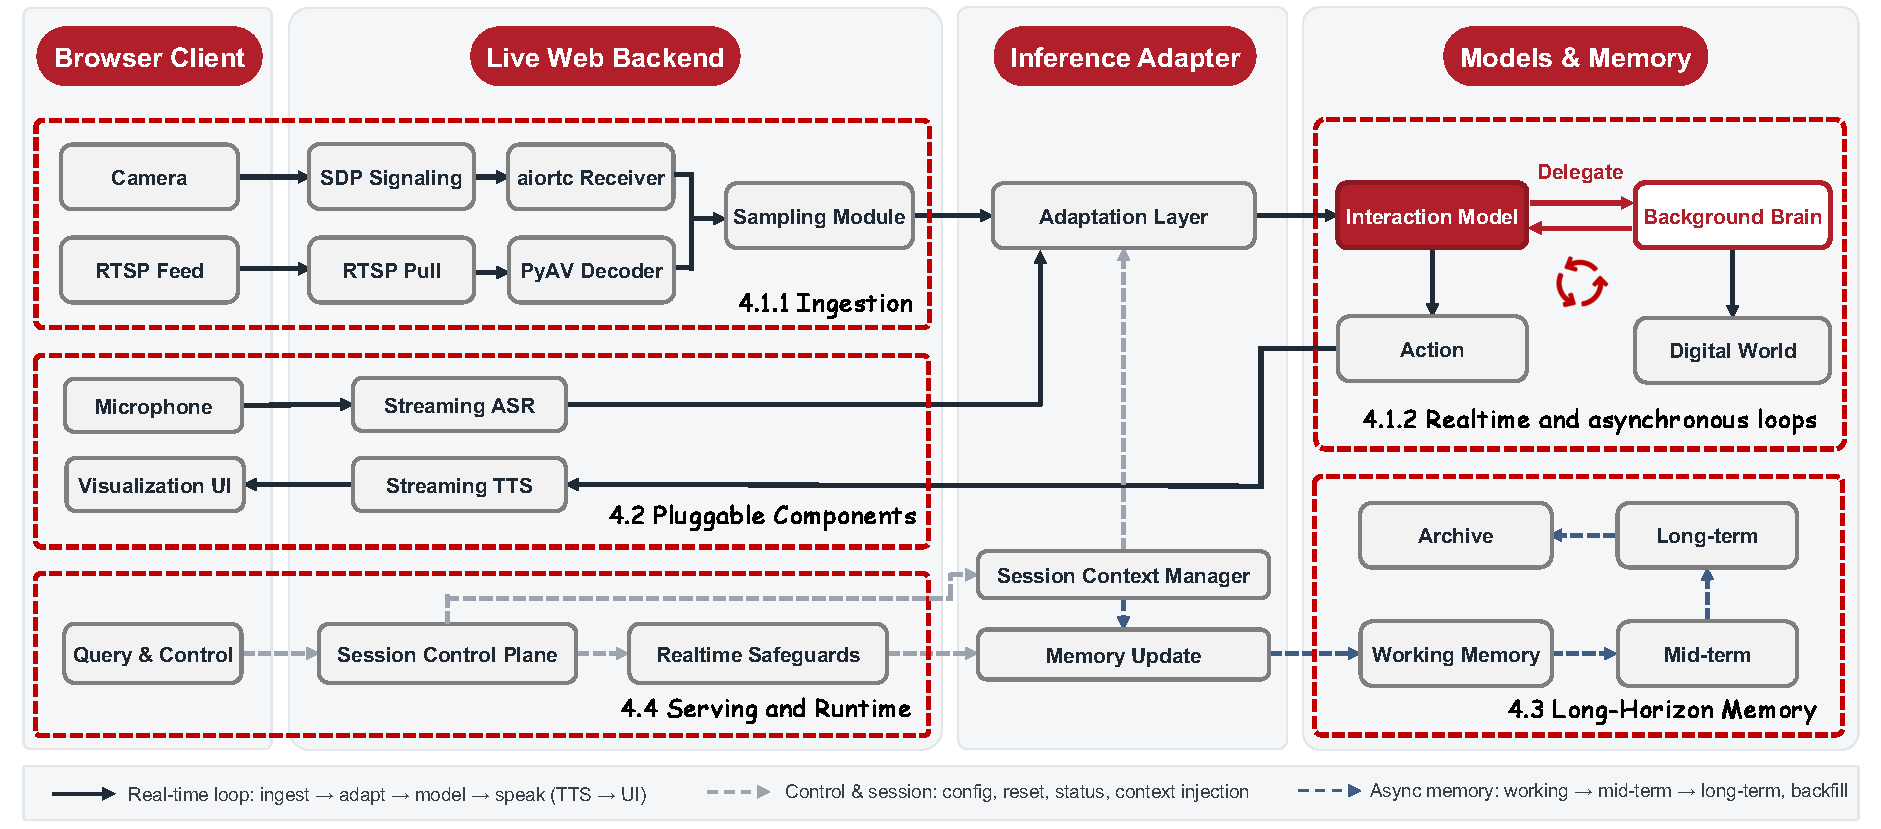
\includegraphics[scale=0.5]{./pic/joyvl-system-architecture.pdf}}
  \caption{Overview of the JoyAI-VL-Interaction System.}
  \label{fig:case}
\end{figure*} 

% \begin{table}[!htbp]
% \centering
% \begin{tabular}{lll}
% \toprule
% Component & Default (out of the box) & Replaceable with \\
% \midrule
% VL interaction model & our post-trained model (§3) & any VLM trained with the §3 recipe \\
% Background brain & \todo{default} & any API, model, or agent you bring \\
% ASR & open-source ASR module & your own ASR API \\
% TTS & open-source TTS module & your own TTS API \\
% Memory & \todo{layered} event memory & your own memory implementation \\
% Visualization UI & built-in UI & your own front end \\
% Serving & vLLM-native & standard vLLM ecosystem \\
% \bottomrule
% \end{tabular}
% \caption{Every component ships with an open-source default and is replaceable. Only the interaction model makes the speak / stay-silent / delegate decision.}
% \label{tab:pluggable}
% \end{table}

\subsection{Two Concurrent Loops: from Seeing to Acting}\label{sec:sys-loops}
The interaction model runs two conversations at once: a real-time loop with the user and an asynchronous loop with the background brain, joined by the model's \texttt{delegate} action.


% \subsection{Two concurrent loops: from seeing to acting}\label{sec:sys-loops}
% The interaction model runs two conversations at once: a real-time loop with the user and an asynchronous loop with the background brain. The real-time loop begins at ingestion. The system receives a continuous, compressed video stream over WebRTC (a browser camera) or RTSP (a livestream feed) and decodes it server-side, with aiortc and PyAV respectively, back into raw frames. A sampling module then downsamples the stream at a fixed interval, 1\,Hz by default and configurable per scenario (for example 2 or 4\,Hz), to balance temporal detail against real-time latency. Each sampled frame is converted to an RGB image, JPEG-encoded, and wrapped as a Base64 data-URL inside an OpenAI-compatible multimodal Chat Completions request, which is the image input the model consumes directly and the same request form our vLLM serving path expects (§\ref{sec:sys-serve}).
\paragraph{\textbf{Ingestion.}} The real-time loop begins at ingestion. A browser client pushes its camera stream to the server through WebRTC SDP negotiation, or submits an RTSP address that the server pulls; the two media paths are received and decoded server-side by aiortc and PyAV respectively, back into raw frames. A sampling module downsamples the stream at a fixed interval, 1\,Hz by default and configurable per scenario, to balance temporal detail against real-time latency. The sampled frames are converted to RGB, JPEG-encoded, and wrapped as Base64 data-URLs, then passed with the active user query into an adaptation layer that assembles an OpenAI-compatible multimodal Chat Completions request, the same request form our vLLM serving path expects (§\ref{sec:sys-serve}).
% \paragraph{\textbf{Ingestion.}} The real-time loop begins at ingestion. The system receives a continuous, compressed video stream over WebRTC (a browser camera) or RTSP (a livestream feed) and decodes it server-side, with aiortc and PyAV respectively, back into raw frames. A sampling module then downsamples the stream at a fixed interval, 1\,Hz by default and configurable per scenario (for example 2 or 4\,Hz), to balance temporal detail against real-time latency. Each sampled frame is converted to an RGB image, JPEG-encoded, and wrapped as a Base64 data-URL inside an OpenAI-compatible multimodal Chat Completions request, which is the image input the model consumes directly and the same request form our vLLM serving path expects (§\ref{sec:sys-serve}).


\paragraph{\textbf{The real-time and asynchronous loops.}} These frames are fed to the model every second, so it always acts on what is happening now rather than on a delayed batch. Together with optional microphone audio transduced by streaming ASR into an active query, they drive the model: at every second it takes one action, to speak, stay silent, or delegate; when it speaks, streaming TTS renders the reply and the visualization UI reflects its state. When it delegates, control passes to the asynchronous loop, in which a background model runs against the background brain to handle slower, more demanding tasks.


% These frames are fed to the model every second, so it always acts on what is happening now rather than on a delayed batch. Together with optional microphone audio transduced by streaming ASR into an active query, they drive the model: at every second it takes one action, to speak, stay silent, or delegate; when it speaks, streaming TTS renders the reply and the visualization UI reflects its state. An asynchronous loop runs against the background brain for slower, harder work, and the \texttt{delegate} action is the seam that joins the two.


\paragraph{\textbf{The background bridge.}} The edge that \texttt{delegate} points to is a background bridge, and the brain behind it defaults to the user's own large-model API while remaining free to be any agent (such as Hermes Agent \cite{hermesagent} and OpenClaw \cite{openclaw} ) the user brings. The scaffold supports this natively and defines a fixed, background-agnostic protocol over text requests and results (§\ref{sec:data}). The bridge exposes a background-agnostic text contract: the foreground emits a tagged query, which the bridge normalizes into a task-id, delegated question, foreground note, and bounded frame snapshot. It runs an isolated model or agent asynchronously under a fixed timeout; expiry is reported as an error event and in-flight work is cancelled on session cleanup. Results return as started/ready/error events, with full artifacts kept off-context and only a bounded digest woven back into the interaction model. Because the background can be an agent, the bridge also closes a loop from seeing to acting: the interaction model observes the physical world and, when warranted, delegates a task the background agent carries out in the digital world. This is the watch-and-do premise of \S\ref{sec:introduction} made operational: see, decide, act, in one system. 

% The edge that \texttt{delegate} points to is a background bridge, and the brain behind it defaults to the user's own large-model API while remaining free to be any API, model, or agent the user brings, from a single model to an agent system such as Hermes or OpenClaw~\todo{confirm names / add citations}. The scaffold supports this natively and defines a fixed, background-agnostic protocol over text requests and results (§\ref{sec:data}), so swapping the background never touches the model. \todo{state the contract: request/result schema, timeout and weave-back policy, multi-background orchestration} Because the background can be an agent, the bridge also closes a loop from seeing to acting: the interaction model observes the physical world and, when warranted, delegates a task the background agent carries out in the digital world, whether placing an order, raising an alert, sending a message, or calling a tool. \todo{name the concrete actions/integrations already wired up} This is the watch-and-do premise of §1 made operational: see, decide, act, in one system.


\subsection{Pluggable Components: Transduction, Visualization, and Your Own Modules}\label{sec:sys-plug}
\paragraph{\textbf{ASR and TTS.}} For speech, we ship a ready-to-run server built on open source ASR \cite{gao2023funasr} and TTS models \cite{du2025cosyvoice}, and users can swap in their own model or API to match their language and preferred voice. These modules only convert modalities; they take no part in the interaction decision. Because speech has duration while generation does not, we predefine a simple rule to keep the two in step: while the previous utterance is still being spoken, the model's next sentence is surfaced as text only and is not synthesized, so audio never piles up behind generation. For high-frequency settings such as live commentary, step-by-step guidance, and real-time subtitle translation, where output is near-continuous, we recommend running with TTS off, and we leave a fuller treatment of this regime to future work.

\paragraph{\textbf{Visualization UI.}} A built-in web interface, adapted from NVIDIA's open-source \texttt{live-vlm-webui}\footnote{\url{https://github.com/nvidia-ai-iot/live-vlm-webui}}, makes the running system visible and controllable.A left-hand configuration panel selects the video source—either a webcam or an RTSP livestream—and sets the sampling cadence, namely the number of frames per inference and the interval between inferences; it also offers a response mode that shifts the model's style from a default balance to more talkative or more aloof. The center pane shows the live stream the model is watching. The right-hand pane is the conversation: it holds the running exchange with the model, including earlier turns, reports per-response and average latency in real time, and accepts either typed messages or spoken input through the microphone (ASR); when the model speaks, its reply is played back automatically through TTS. The interface doubles as a debugging and trust surface for sensitive deployments, and it can be replaced with a custom front end.

\paragraph{\textbf{Bring your own modules.}} Beyond these defaults, the system is open to user-supplied modules that enrich what the assistant perceives or remembers. As one example, a face-recognition module can let the assistant remember who you are and recognize when a particular friend or family member walks into the scene, opening up more personal and engaging interactions. There is a larger reason we open all of this. Turn-based interaction is a long-settled range, refined over years, with a vast ecosystem of systems and optimizations built up around it; VL interaction models, by contrast, have barely begun. By releasing the full stack, we hope to open a first breach for interaction models among those established peaks, and we invite the community to explore with us what this still-young way of working with AI can become.


\subsection{Long-Horizon Memory}\label{sec:sys-mem}
Long-horizon presence needs a memory whose footprint does not grow without bound as a stream runs for hours, and whose contents form a shared context read by both the streaming model and the background brain. We meet this with a pluggable hierarchical memory built on our prior work~\cite{yao2026harnessingstreamingvideowild}, organized into tiers at increasing compression.
We organize the context into a three-tier hierarchy that partitions the stream into: (i) a \textit{short-term memory} retaining the most recent $T_s$ seconds as raw vision tokens; (ii) a \textit{mid-term memory} holding up to $M$ textual summaries of past short-term chunks, covering $T_m = M T_s$ seconds at moderate compression; and (iii) a \textit{long-term memory} storing up to $L$ aggressively compressed blocks, each consolidated from $M$ consecutive mid-term summaries and thus spanning $T_l = L M T_s$ seconds.
Alongside these visual tiers, a dialogue memory keeps past queries and answers coherent across time. The consolidation steps run asynchronously, ahead of each boundary, so they hide behind mainline inference and never stall the real-time loop, and together the tiers reach up to roughly two hours of context. Because each tier above the buffer is stored as text, the memory also forms a stable per-chunk prefix that the serving path of §\ref{sec:sys-serve} can cache and reuse; it is designed for exactly this, and it remains fully pluggable, swappable for any external memory a deployment prefers.


% Long-horizon presence needs a memory whose footprint does not grow without bound as a stream runs for hours, and whose contents form a shared context read by both the streaming model and the background brain. We meet this with a pluggable hierarchical memory built on our prior work~\cite{yao2026harnessingstreamingvideowild}, organized into tiers at increasing compression. The most recent frames (short-term memory) stay available raw in the live buffer, preserving fine detail for the present. Every 100 seconds, a mid-term step condenses the accumulated frames into a single text paragraph, a chunk summary, trading vision tokens for far cheaper text. Every 500 seconds, a long-term step fuses these chunk summaries into a durable, compressed memory, merging overlapping content and arranging causally related events into a coherent timeline. Alongside these visual tiers, a dialogue memory keeps past queries and answers coherent across time. The consolidation steps run asynchronously, ahead of each boundary, so they hide behind mainline inference and never stall the real-time loop, and together the tiers reach up to roughly two hours of context. Because each tier above the buffer is stored as text, the memory also forms a stable per-chunk prefix that the serving path of §\ref{sec:sys-serve} can cache and reuse; it is designed for exactly this, and it remains fully pluggable, swappable for any external memory a deployment prefers.

% Two points keep this consistent with the rest of the system. First, the tiers only store and retrieve; they never decide when to speak, so memory sits on the orchestration side of \S\ref{sec:sys-arch} rather than touching the model's interaction decision, and it stays fully pluggable, swappable for any external memory a deployment prefers. Second, we keep two easily-conflated quantities distinct: the duration over which the system runs at low latency is a serving property bounded by the path of \S\ref{sec:sys-serve}, whereas the time span the memory can address is bounded by the formula above. A deployment can sustain hours of continuous low-latency operation while the memory reaches back across a different, longer horizon, and we report each separately. \todo{state the two numbers, e.g. sustained low-latency runtime vs. addressable memory span}

% \paragraph{\textbf{Face.}}  \todo{bring more imagination}



% \paragraph{\textbf{Visualization UI.}} A built-in interface surfaces what the model is watching, its current action (speak, stay silent, or delegate), the background's progress, and memory activity. \todo{confirm what the UI surfaces} It is both a product surface and a debugging and trust tool for sensitive settings, and it can be replaced with a custom front end. 

% \paragraph{\textbf{Visualization UI.}} A built-in interface shows the live stream the model is watching, alongside the running exchange between the user and the model, both the earlier turns and the current one. From the interface the user can choose the input source, a camera stream or a livestream feed, both adapted out of the box, and adjust the ingestion frame rate (FPS) on the fly to trade visual detail against cost; when the model speaks, its reply is played back automatically through TTS. The interface doubles as a debugging and trust surface for sensitive deployments, and it can be replaced with a custom front end.

\subsection{Serving and Runtime}\label{sec:sys-serve}
\paragraph{\textbf{vLLM-native serving.}}
Hours of continuous video defeat the obvious serving strategies. Recomputing attention over the full history saturates the context window within a few hundred seconds; a sliding window bounds the context but breaks prefix reuse, since successive steps no longer share a common prefix, so an engine's prefix cache buys nothing and latency plateaus above the real-time budget; token pruning has the same problem. Most streaming-video methods inherit one of these and, built on plain Transformers, stay incompatible with efficient engines such as vLLM \cite{kwon2023efficientmemorymanagementlarge} and SGLang \cite{zheng2024sglangefficientexecutionstructured}, which is much of why they remain in the lab. We instead designed the memory system around prefix reuse so that vLLM serves it directly: the text memory of §\ref{sec:sys-mem} is prefilled once per chunk into a KV cache, and at every subsequent step only the newly observed frames and the previous reply are computed, while the memory and earlier in-chunk turns are reused without recomputation. AdaCodec (§\ref{sec:arch}) further shrinks each predictable frame to about sixteen tokens, keeping per-step work small. Building the memory this way is precisely what lowers the bar to deployment: the system sustains over two hours of continuous video at sub-second end-to-end latency on standard vLLM. 

% Running on standard vLLM has a second payoff: existing inference infrastructure serves the system directly, with close to zero operational learning curve. This contrasts with a bespoke serving stack (TML's SGLang work) and with a multi-module cascade (the Doubao pipeline), and it is much of what separates a deployable interaction system from a prototype that never leaves an offline benchmark.

\paragraph{\textbf{Stateful sessions.}} The runtime is organized around server-side sessions. Control messages, configuration updates, session resets, and state synchronization, travel as JSON over WebSocket or HTTP and carry a \texttt{session\_id}, while the server keeps each session's video context, question-and-answer trajectory, and memory state. When a request is assembled, this maintained context is injected automatically into the Chat Completions request, so a single round of client-server communication carries only the instantaneous observation, and all long-horizon context management lives at the backend. This is also what makes the prefix reuse above possible: the injected context is precisely the stable per-chunk prefix the engine caches and reuses.

\paragraph{\textbf{Real-time robustness.}} To hold latency steady under load, the runtime places timeouts, reconnection, and cancellation across connection setup, the WebSocket channel, RTSP signaling, and the auxiliary audio and video channels, and a session-level lock keeps requests from piling up; when it must, it drops stale frames or backfills late results into the correct interaction history by inference sequence number. The adaptation layer routes each request by its model identifier to the corresponding VLM service, runs the mid-term and long-term memory consolidation of §\ref{sec:sys-mem} in parallel, and returns a standard JSON response.


\paragraph{\textbf{Everything is open.}} The model recipe, the background bridge, ASR/TTS, memory, orchestration, the visualization UI, and the vLLM serving path can all be replaced or extended in the repository. Releasing the model recipe and the complete system together is the whole point: from a single repository, anyone can stand up their own present, self-directed real-world assistant. 
% // The full open-source manifest, its value to the community, and application scenarios are detailed in §6.
\section{Experiments}
\label{sec:experiments}
% \subsection{Benchmark}
\subsection{Benchmark}\label{sec:benchmark}
We evaluate JoyAI-VL-Interaction not on offline video-understanding benchmarks but against the real, deployed products people would actually reach for, in the live, event-driven setting this paper is about. Concretely, we compare it head-to-head with the in-app video-call assistants of Doubao and Gemini, today's most mature and recognizable real-time multimodal products (\S\ref{sec:product}). We choose six everyday scenarios that fall squarely in the advantage zone of the interaction-model paradigm: settings that demand being present, acting unprompted at the right moment, and tracking events over time, precisely what a turn-based product, waiting to be addressed, is structurally unequipped to deliver however fast it answers once asked.

\paragraph{\textbf{Scenarios.}} The six scenarios are: (1) \textit{monitoring and alerting}, flagging an event the instant it occurs; (2) \textit{real-time counting} of objects or events over time; (3) \textit{real-time translation} of on-screen content; (4) \textit{time awareness}, acting on its own sense of elapsed time, for instance speaking once every few seconds on request or timing how long an activity lasts; (5) \textit{live commentary and guidance}, narrating or walking the user through an unfolding scene at the right moments; and (6) \textit{long-horizon memory}, answering about something seen far earlier in the stream. Underneath the six lie the three capabilities that define an interaction model: real-time operation, proactive response driven by what it sees, and long-horizon memory. The six are thus not an arbitrary set but a sampling of these axes, and the same capabilities reach far beyond this benchmark, into AI glasses, assistance for the blind, security monitoring, home robots, home and elder care, vision-grounded chat and companionship apps, live sports commentary, and delegation to background agents, among others. All are settings where being present and acting at the right moment is the whole task, the dimension on which turn-based products structurally fall short, so the six probe the paradigm gap itself rather than any single product feature.
The six scenarios comprise 58 cases in total: 10 each for monitoring, counting, translation, and time awareness, and 9 each for commentary and memory. 
The cases are drawn mostly from public footage on the web, with a few recorded by us.
% and each is replayed identically to all three systems: most are streamed in over RTSP, with the server pulling the address and decoding it back into raw frames, while a few are delivered as a camera stream to the server through WebRTC SDP negotiation (\S\ref{sec:system}); either path feeds the systems exactly as in live deployment, so all three see the same frames at the same pace and the comparison turns only on how each one responds.

\paragraph{\textbf{Baselines.}} Our baselines are the video-call features of the Doubao and Gemini apps, the products we single out in \S\ref{sec:product} as turn-based at the core, each evaluated as it is actually deployed to end users. We use the app versions current in late May and early June 2026, and drive each product with the same input under matched conditions. We run JoyAI-VL-Interaction through our own system (\S\ref{sec:system}) and compare it against each baseline separately, pairwise. 
The JoyAI-VL-Interaction system uses a three-tier memory with $T_s=100$\,s, $M=5$, and $L=15$ (\S\ref{sec:sys-mem}).
At evaluation time, our JoyAI-VL-Interaction system simulates offline videos as a live streaming source over RTSP, served by MediaMTX.
Since Doubao and Gemini expose no system-level API, we drive them through their apps: we play the same video to each and pose identical questions at matched timestamps.


\paragraph{\textbf{Protocol and metric.}} For every case, human raters score each system on two equally important axes: \textit{quality}, whether the response is correct, relevant, and well-formed; and \textit{timing}, whether it arrives at the right moment, neither premature nor late, and whether the system stays silent when nothing is worth saying. Each axis is rated on a three-level scale, good, fair, or poor, and a system's score for the case is the equal-weight average of its two axis ratings. The timing axis is the crux of the event-driven setting and the one turn-based products structurally struggle with (\S\ref{sec:introduction}). To reduce bias, system identities are hidden from raters and the presentation order is randomized. Five raters carry out the ratings, all educated to at least the university level and working as researchers in LLMs, and inter-rater agreement is high. For each case we then compare the two systems' weighted-average scores, which gives a win, tie, or loss for JoyAI-VL-Interaction. We report the per-scenario and overall \textit{win rate}, the fraction of comparisons it wins, against Doubao and against Gemini respectively, alongside the tie and loss rates; a tie counts as neither a win nor a loss.



\begin{table}[!htbp]
\centering
\renewcommand{\arraystretch}{1.3}
\begin{tabular}{lccc}
\toprule
\textbf{Scenario} & \textbf{JoyAI-VL-Interaction} & \textbf{Tie} & \textbf{Doubao} \\
\midrule
Monitoring and alerting      & \textbf{100.0\%} & 0.0\%  & 0.0\%  \\
Real-time counting                & \textbf{70.0\%}  & 30.0\% & 0.0\%  \\
Real-time translation        & \textbf{80.0\%}  & 20.0\% & 0.0\%  \\
Time awareness               & \textbf{80.0\%}  & 10.0\% & 10.0\% \\
Live commentary and guidance & \textbf{55.6\%}  & 22.2\% & 22.2\% \\
Long-horizon memory          & \textbf{77.8\%}  & 22.2\% & 0.0\%  \\
\midrule
\textbf{Overall}             & \textbf{77.6\%}  & \textbf{17.2\%} & \textbf{5.2\%} \\
\bottomrule
\end{tabular}
\caption{Head-to-head human evaluation, JoyAI-VL-Interaction versus Doubao's in-app video-call assistant.}
\end{table}


\begin{table}[!htbp]
\centering
\renewcommand{\arraystretch}{1.3}
\begin{tabular}{lccc}
\toprule
\textbf{Scenario} & \textbf{JoyAI-VL-Interaction} & \textbf{Tie} & \textbf{Gemini} \\
\midrule
Monitoring and alerting      & \textbf{100.0\%} & 0.0\%  & 0.0\%  \\
Real-time counting                & \textbf{100.0\%} & 0.0\%  & 0.0\%  \\
Real-time translation        & \textbf{100.0\%} & 0.0\%  & 0.0\%  \\
Time awareness               & \textbf{50.0\%}  & 40.0\% & 10.0\% \\
Live commentary and guidance & \textbf{100.0\%} & 0.0\%  & 0.0\%  \\
Long-horizon memory          & \textbf{77.8\%}  & 22.2\% & 0.0\%  \\
\midrule
\textbf{Overall}             & \textbf{87.9\%}  & \textbf{10.3\%} & \textbf{1.7\%} \\
\bottomrule
\end{tabular}
\caption{Head-to-head human evaluation, JoyAI-VL-Interaction versus Gemini's in-app video-call assistant.}
\end{table}




\subsection{Results and Case Study}

\paragraph{\textbf{Experimental Results.}}
Across both comparisons JoyAI-VL-Interaction is the preferred system by a wide margin, and in every scenario it wins more comparisons than it loses. Against Doubao it is preferred in 77.6\% of cases, ties 17.2\%, and loses only 5.2\%; against Gemini the margin is wider still, at 87.9\% wins, 10.3\% ties, and just 1.7\% losses. The two baselines, in other words, almost never come out ahead overall.

Our model's clearest advantage falls exactly on the vision-driven, time-critical scenarios that define the paradigm. In monitoring and alerting, the purest test of catching an event the instant it occurs, it wins every single comparison against both baselines (100\%). Real-time translation and fast counting are similarly lopsided: it sweeps both at 100\% against Gemini, and wins 80\% and 70\% against Doubao with no losses at all. These are precisely the settings where being present and acting at the right moment is the whole task, and they are where our margins are largest, which is the central claim of the benchmark borne out in the numbers. Long-horizon memory is also strong, at 77.8\% against each. Part of this margin reflects a structural limit of the baselines rather than a single weak answer: in video-call mode Doubao automatically hangs up after about five minutes with no voice input, and Gemini at around two minutes fifteen seconds, so in around half of the memory cases the question we ask falls past these cutoffs and neither baseline is even present to respond, scoring nothing. However, on the shorter cases that stay within their session limits, our model still wins or ties. We credit it to our long-horizon memory design: a mid-term and a long-term step that continuously compress, merge, and organize what the model has seen, so that information from far earlier in the stream is still at hand when a question finally arrives.

Where the baselines do gain ground, they do so for different reasons, and never on timing. Doubao's main foothold is live commentary and guidance, where it wins 22.2\% of cases and ties another 22.2\% against our 55.6\%. Its edge here is one of quality rather than timing: a larger model scale gives it broader knowledge, richer style, and more varied phrasing, which lands it in the comfort zone of some narration tasks. Its timing, in fact, is a weakness. On commentary, however, its timing works against it: the responses are temporally erratic, arriving too frequently in some passages and too sparsely in others, because its periodic external trigger has no means of judging when a remark is genuinely warranted. This corroborates our central design principle: deciding when to respond must be a native capability of the model, learned and judged internally, rather than a behavior supplied by an external trigger. Doubao therefore prevails on these cases only when its quality advantage is large enough to offset its weaker timing under the equal-weight scoring. Our own losses, in turn, are confined to quality: the model occasionally hallucinates during commentary, a limitation we attribute primarily to its parameter scale and regard as a principal direction for future work.
Gemini's single foothold is time awareness, the closest-contested axis against it, where it ties 40\% of cases and wins 10\%, holding our win rate to 50\%, while on every other scenario it fails to win a single comparison. The reason is specific to this scenario: some time-awareness cases are user-triggered, with the question asked only after the relevant moment has passed, so the real-time demand is low. On these ask-after-the-fact questions, Gemini's strong underlying model answers well on quality alone.
In both cases the baselines close the gap only where timing pressure is lowest, winning on raw answer quality or on questions that no longer require a split-second response, and they fall furthest behind exactly where a reply must land at the right moment.



\paragraph{\textbf{Case Study.}}
To make the quantitative gap concrete, we walk through six representative cases; the full side-by-side video comparisons are available in our blog.\footnote{\url{https://joyai-vl-video-future-academy-jd.github.io/JoyAI-VL-Interaction}} Each contrasts JoyAI-VL-Interaction with Doubao's and Gemini's in-app video-call assistants on identical input.

In the \textit{Fall Detection Alert} case (02 Monitoring and alerting in the blog), a person collapses on camera. JoyAI-VL-Interaction raises the alert at the instant of the fall, whereas Doubao reacts four to five seconds later, and Gemini explicitly concedes that it is unable to monitor the scene at all. The lag is not incidental: it is the polling interval of an external trigger surfacing as latency on an event that allows no delay.
The \textit{Real-time Dart Throw Counting} case (05 Real-time counting in the blog) tests sustained, event-locked counting. JoyAI-VL-Interaction increments its count exactly as each dart strikes the board, registering all six throws on time, while Doubao counts only two and with noticeable delay, and Gemini offers a single ``let me check'' before falling silent.
The \textit{Street Interview Translation} case (01 Real-time translation in the blog) probes continuity, with the task being to translate the interview's on-screen subtitles in real time rather than its audio. JoyAI-VL-Interaction translates the speech continuously and stays accurate even when Chinese pinyin appears in the on-screen subtitles, whereas both Doubao and Gemini translate only what was visible at the moment the request was issued and then stop, treating an ongoing task as a single turn.
The \textit{Timed Cooking Scene} case (06 Time awareness in the blog) asks the system to signal once a twenty-second interval has elapsed, a direct probe of an internal sense of time. JoyAI-VL-Interaction is off by only one to two seconds; Doubao fails to signal at the mark altogether, and Gemini does so only at around forty seconds, roughly double the target.
The \textit{Pet Livestream Commentary} case (04 Live commentary in the blog) plays a continuous stream of short clips of different pets, requiring the model to keep pace with the changing scene and to recognize and narrate each animal's emotional state. JoyAI-VL-Interaction narrates each pet as it appears, whereas Doubao cannot keep up, describing only three of thirteen and inaccurately at that, and Gemini comments just once, and only when prompted.
The \textit{Phone App Delegation} case (09 Agent delegation in the blog) illustrates a capability the baselines do not offer at all: when a phone's app interface appears on screen, the model is asked to produce HTML that renders a similar screen. JoyAI-VL-Interaction recognizes that this exceeds real-time inference, hands the task to the background model, and returns working HTML reproducing the observed interface, all without leaving the live session.


\paragraph{\textbf{Emergent capabilities.}}
Two further cases are more striking still, in that they exercise capabilities the model was never trained for. In the \textit{Shopping App Guidance} case (03 App guidance in the blog), the user pursues a shopping goal while swiping through a phone's screens. JoyAI-VL-Interaction responds promptly and narrates in step with each swipe, guiding the user to the intended item, whereas neither Doubao nor Gemini reacts proactively or in real time, describing only a few of the screens first shown. Notably, our training data contains no app-interface video of any kind: the ability to follow a changing interface is one the model acquired on its own, generalizing to a domain it never saw.
In the \textit{Travel Scene Commentary} case (04 Live commentary in the blog), the system is asked to narrate once every four seconds. JoyAI-VL-Interaction holds to this cadence throughout and keeps the commentary substantively strong; Doubao narrates only the opening scene for some twenty seconds and ignores the four-second instruction entirely, while Gemini, though asked in Chinese, replies in English and comments only once. The task combines two abilities, timed action and live commentary, that never co-occur in our training data: the model composes them at inference time, an emergent crossing of capabilities rather than a pattern it was shown.

Across these cases the same factor separates JoyAI-VL-Interaction from systems many tens or even hundreds of times its size: timing. By making the decision of when to respond a native, learned capability of the model rather than a behavior imposed by an external trigger, JoyAI-VL-Interaction acts at the moment each event demands, where larger but turn-based or polling-based systems arrive late, stop after a single turn, or never engage. Moreover, its compact size imposes no ceiling on what it can ultimately handle: when a problem genuinely calls for a more powerful model, JoyAI-VL-Interaction does not attempt to answer it inline but delegates it, dispatching the hard subtask to a background model through an asynchronous request and folding the result back in once it returns, all while remaining present with the user in real time. A compact 8B model thus pairs real-time, well-timed presence with on-demand access to heavier reasoning, which we regard as the decisive reason it can outperform far larger models and mature products on the dimension that matters most in the streaming setting.


% \subsection{Emergent capabilities: behaviors we never trained for}\label{emergent}



\subsection{Limitations}\label{sec:limitations}
A fair reading of our comparison has to start with scale. The two video-call assistants we evaluate against are powered by far larger models, Seed 2.0 behind Doubao and Gemini-3.1-flash-live behind Gemini, and both are mature products tuned over time against real users and use cases. JoyAI-VL-Interaction, by comparison, is a compact 8B-scale model. We therefore expect, and do not claim otherwise, that on general turn-based ability these products are stronger than ours: broader world knowledge, a more polished one-on-one chat experience, and greater robustness on complex or rarely seen inputs.

Our claim is narrower, and we think more telling. In the six event-driven scenarios this paper targets, the ones that turn on real-time presence, proactive interaction, and a sense of time, and that already carry rich deployment value, a far smaller model holds a natural advantage simply by being an interaction model rather than a turn-based one. That a compact, open model can outperform far larger and heavily optimized products precisely in this regime is, to us, the point: interactivity is worth scaling as a capability in its own right, and it begins to pay off well before enormous scale.

% The training data behind this release is, by deliberate choice, still at an early stage. We have not yet tuned its mixture or scaled it to the volume we ultimately intend, and a further round of data cleaning remains. One consequence is already evident in our evaluation: the commentary data is comparatively sparse, which is the principal cause of the occasional hallucination the model exhibits during live narration (\S\ref{sec:experiments}). We nonetheless release the model at this stage. Even now it exhibits capabilities we never trained for, and the emergence of these behaviors persuaded us that the approach merited release to the community rather than awaiting a fully optimized data recipe. A subsequent version will tune the data mixture and scale the corpus; in the interim, it is the data-construction methodology itself, rather than this particular corpus, that we expect others can most readily adapt and extend.

Both the data and the evaluation behind this release are, by deliberate choice, still at an early stage. On the data side, we have not yet tuned the mixture or scaled it to the volume we ultimately intend, and a further round of cleaning remains; one consequence is already visible in our results, where the comparatively sparse commentary data, together with the model's compact scale, is the main cause of the occasional hallucination during live narration (\S\ref{sec:experiments}). The evaluation is similarly preliminary, six scenarios and 58 human-rated cases against two products, rather than the larger, more fine-grained study we ultimately want. We release at this stage regardless, and the reason is the same for both: even with this early data and this limited evaluation, the model already exhibits interaction capabilities we never explicitly trained for, and watching them emerge convinced us, more than any single number could, that interactivity is a direction worth scaling in its own right. That conviction is exactly why we would rather put the model, the recipe, and the system into the community's hands now than hold them back for a polished data recipe and a larger benchmark: we are eager to scale this direction together rather than alone. A subsequent version will tune the data mixture, scale the corpus, and report a broader and more systematic evaluation; in the interim, it is the data-construction methodology and the approach itself, rather than this particular corpus or benchmark, that we expect others can most readily adapt and extend. These limitations also chart the road ahead: closing the gap in general ability and robustness, widening the set of scenarios, and pushing further on what an interaction model can do.

% Our evaluation is likewise still limited in scale, six scenarios and 58 human-rated cases against two products; a future version will broaden the scenarios, enlarge the case set, add more baselines, and report a more fine-grained and systematic evaluation.

% These limitations also chart the road ahead. Closing the gap in general ability and robustness, widening the set of scenarios, and pushing on what an interaction model can do are exactly the directions we hope to pursue together with the community; we release JoyAI-VL-Interaction in full so that anyone can help build out and extend its capabilities.
% \section{Conclusion}

\section{Conclusion}\label{sec:conclusion}
We set out to move large models past the turn-based paradigm, in which a model opens its eyes only when it is addressed, toward genuine streaming interaction, in which the model is present in the world and decides for itself when to act. To that end we release, to our knowledge, the first open vision-driven interaction model, together with everything needed to build on it: the time-aligned data, the training recipe, the 8B model, and a complete, deployable system.

At the center is a single conviction, that interactivity should scale as a capability of the model itself rather than be simulated by a harness around it. Scaling interactivity means scaling three things at once: the model's freedom to speak on its own when a moment is worth a word, its ability to interact in real time, and its sense of elapsed time. As these grow, a model behaves less like a tool that waits to be queried and more like a participant that is simply present, watching what is happening and responding as a person would. We see this as a direction of scaling in its own right, alongside the scaling of intelligence, and one that brings models closer to being genuinely present in human settings.

Across the streaming scenarios we study, we already see early signs that an interaction model carries natural advantages for real deployment, from monitoring and live narration to step-by-step guidance and companionship. The moment we are reaching for is an everyday one: you come home worn out after a long day, and before you have said anything, a quiet voice notices and offers, ``I can see you're tired; today must have been hard on you.'' Presence like that, given unasked, is what an interaction model makes possible and a turn-based one, waiting to be addressed, never can. Much remains open in both the model and the system, and we have released the whole stack openly to lower the barrier and accelerate this shift. Turn-based models, products, and optimizations have been built up over many years, while vision-driven interaction models are only beginning; if this release opens even a first foothold for them among those long-settled peaks, and draws others into building it with us, it will have done its job. We invite the community to explore, with us, what a model that is truly present in the world can become. 

% \section{Acknowledgment}

% ddd


\bibliographystyle{assets/plainnat}
\bibliography{references}

\section{Appendix}
\subsection{Training Data Example}
\begin{lstlisting}[language=json,caption={Example of monitoring and alerting.}, label={lst:example1}]
      {
        "role": "user",
        "content": "Alert me whenever a physical confrontation happens. \n<0.0 seconds>\n<image>\n<image>"
      },
      {
        "role": "assistant",
        "content": "</silence>"
      },
      {
        "role": "user",
        "content": "<1.0 seconds>\n<image>\n<image>"
      },
      {
        "role": "assistant",
        "content": "</silence>"
      },
      {
        "role": "user",
        "content": "<2.0 seconds>\n<image>\n<image>"
      },
      {
        "role": "assistant",
        "content": "</silence>"
      },
      {
        "role": "user",
        "content": "<3.0 seconds>\n<image>\n<image>"
      },
      {
        "role": "assistant",
        "content": "</silence>"
      },
      {
        "role": "user",
        "content": "<4.0 seconds>\n<image>\n<image>"
      },
      {
        "role": "assistant",
        "content": "</response> A physical confrontation is happening."
      },
      {
        "role": "user",
        "content": "<5.0 seconds>\n<image>\n<image>"
      },
      {
        "role": "assistant",
        "content": "</response> A physical confrontation is happening."
      },
      {
        "role": "user",
        "content": "<6.0 seconds>\n<image>\n<image>"
      },
      {
        "role": "assistant",
        "content": "</response> A physical confrontation is happening."
      },
      {
        "role": "user",
        "content": "<7.0 seconds>\n<image>\n<image>"
      },
      {
        "role": "assistant",
        "content": "</response> A physical confrontation is happening."
      },
      {
        "role": "user",
        "content": "<8.0 seconds>\n<image>\n<image>"
      },
      {
        "role": "assistant",
        "content": "</response> A physical confrontation is happening."
      },
      {
        "role": "user",
        "content": "<9.0 seconds>\n<image>\n<image>"
      },
      {
        "role": "assistant",
        "content": "</response> A physical confrontation is happening."
      },
      {
        "role": "user",
        "content": "<10.0 seconds>\n<image>\n<image>"
      },
      {
        "role": "assistant",
        "content": "</silence>"
      },
      ...
\end{lstlisting}


\begin{lstlisting}[language=json,caption={Example of multi-turn casual chat.}, label={lst:example2}]
      ...
      {
        "role": "user",
        "content": "Is the person cleaning the desk?\n<7.0 seconds>\n<image>\n<image>\n<image>\n<image>"
      },
      {
        "role": "assistant",
        "content": "</response> Yep, definitely cleaning the desk! Getting all the dust off that pink surface."
      },
      {
        "role": "user",
        "content": "<8.0 seconds>\n<image>\n<image>\n<image>\n<image>"
      },
      {
        "role": "assistant",
        "content": "</silence>"
      },
      {
        "role": "user",
        "content": "<9.0 seconds>\n<image>\n<image>\n<image>\n<image>"
      },
      {
        "role": "assistant",
        "content": "</silence>"
      },
      {
        "role": "user",
        "content": "<10.0 seconds>\n<image>\n<image>\n<image>\n<image>"
      },
      {
        "role": "assistant",
        "content": "</silence>"
      },
      {
        "role": "user",
        "content": "<11.0 seconds>\n<image>\n<image>\n<image>\n<image>"
      },
      {
        "role": "assistant",
        "content": "</silence>"
      },
      {
        "role": "user",
        "content": "<12.0 seconds>\n<image>\n<image>\n<image>\n<image>"
      },
      {
        "role": "assistant",
        "content": "</silence>"
      },
      {
        "role": "user",
        "content": "What are they doing with the pillow?\n<13.0 seconds>\n<image>\n<image>\n<image>\n<image>"
      },
      {
        "role": "assistant",
        "content": "</response> They're picking up the pillow and moving it around, maybe fluffing it or putting it somewhere."
      },
      {
        "role": "user",
        "content": "<14.0 seconds>\n<image>\n<image>\n<image>\n<image>"
      },
      {
        "role": "assistant",
        "content": "</silence>"
      },
      {
        "role": "user",
        "content": "<15.0 seconds>\n<image>\n<image>\n<image>\n<image>"
      },
      {
        "role": "assistant",
        "content": "</silence>"
      },
      {
        "role": "user",
        "content": "<16.0 seconds>\n<image>\n<image>\n<image>\n<image>"
      },
      {
        "role": "assistant",
        "content": "</silence>"
      },
      {
        "role": "user",
        "content": "<17.0 seconds>\n<image>\n<image>\n<image>\n<image>"
      },
      {
        "role": "assistant",
        "content": "</silence>"
      },
      {
        "role": "user",
        "content": "Why is the person holding keys now?\n<18.0 seconds>\n<image>\n<image>\n<image>\n<image>"
      },
      {
        "role": "assistant",
        "content": "</response> Hmm, they seem to be fiddling with the keys on the desk. Maybe checking or organizing them?"
      },
      ...
\end{lstlisting}


\begin{lstlisting}[language=json,caption={Example of background model delegation.}, label={lst:example3}]
      ...
      {
        "role": "user",
        "content": "<29.0 seconds>\n<image>\n<image>\n<image>\n<image>"
      },
      {
        "role": "assistant",
        "content": "</silence>"
      },
      {
        "role": "user",
        "content": "What are those two guys doing near the boat?\n<30.0 seconds>\n<image>\n<image>\n<image>\n<image>"
      },
      {
        "role": "assistant",
        "content": "</response> Looks like they're walking alongside it, probably supervising or guiding as it gets lifted."
      },
      {
        "role": "user",
        "content": "<31.0 seconds>\n<image>\n<image>\n<image>\n<image>"
      },
      {
        "role": "assistant",
        "content": "</silence>"
      },
      {
        "role": "user",
        "content": "<32.0 seconds>\n<image>\n<image>\n<image>\n<image>"
      },
      {
        "role": "assistant",
        "content": "</silence>"
      },
      {
        "role": "user",
        "content": "<33.0 seconds>\n<image>\n<image>\n<image>\n<image>"
      },
      {
        "role": "assistant",
        "content": "</silence>"
      },
      {
        "role": "user",
        "content": "<34.0 seconds>\n<image>\n<image>\n<image>\n<image>"
      },
      {
        "role": "assistant",
        "content": "</silence>"
      },
      {
        "role": "user",
        "content": "<35.0 seconds>\n<image>\n<image>\n<image>\n<image>"
      },
      {
        "role": "assistant",
        "content": "</silence>"
      },
      {
        "role": "user",
        "content": "<36.0 seconds>\n<image>\n<image>\n<image>\n<image>"
      },
      {
        "role": "assistant",
        "content": "</silence>"
      },
      {
        "role": "user",
        "content": "<37.0 seconds>\n<image>\n<image>\n<image>\n<image>"
      },
      {
        "role": "assistant",
        "content": "</silence>"
      },
      {
        "role": "user",
        "content": "Why does this boat hoist use a four-point sling configuration with spreader bars rather than lifting from a single central point, and how does the load distribution prevent hull deformation in fiberglass vessels?\n<38.0 seconds>\n<image>\n<image>\n<image>\n<image>"
      },
      {
        "role": "assistant",
        "content": "</response> Let me check the engineering principles behind that hoist design. </delegation> Explain the structural engineering principles of four-point boat lifting slings, load distribution, and hull deformation prevention in fiberglass boat hoists."
      },
      {
        "role": "user",
        "content": "<39.0 seconds>\n<image>\n<image>\n<image>\n<image>"
      },
      {
        "role": "assistant",
        "content": "</silence>"
      ...
\end{lstlisting}
\end{document}
